\chapter{Abbildungen}
\begin{figure}[H]
  \centering
  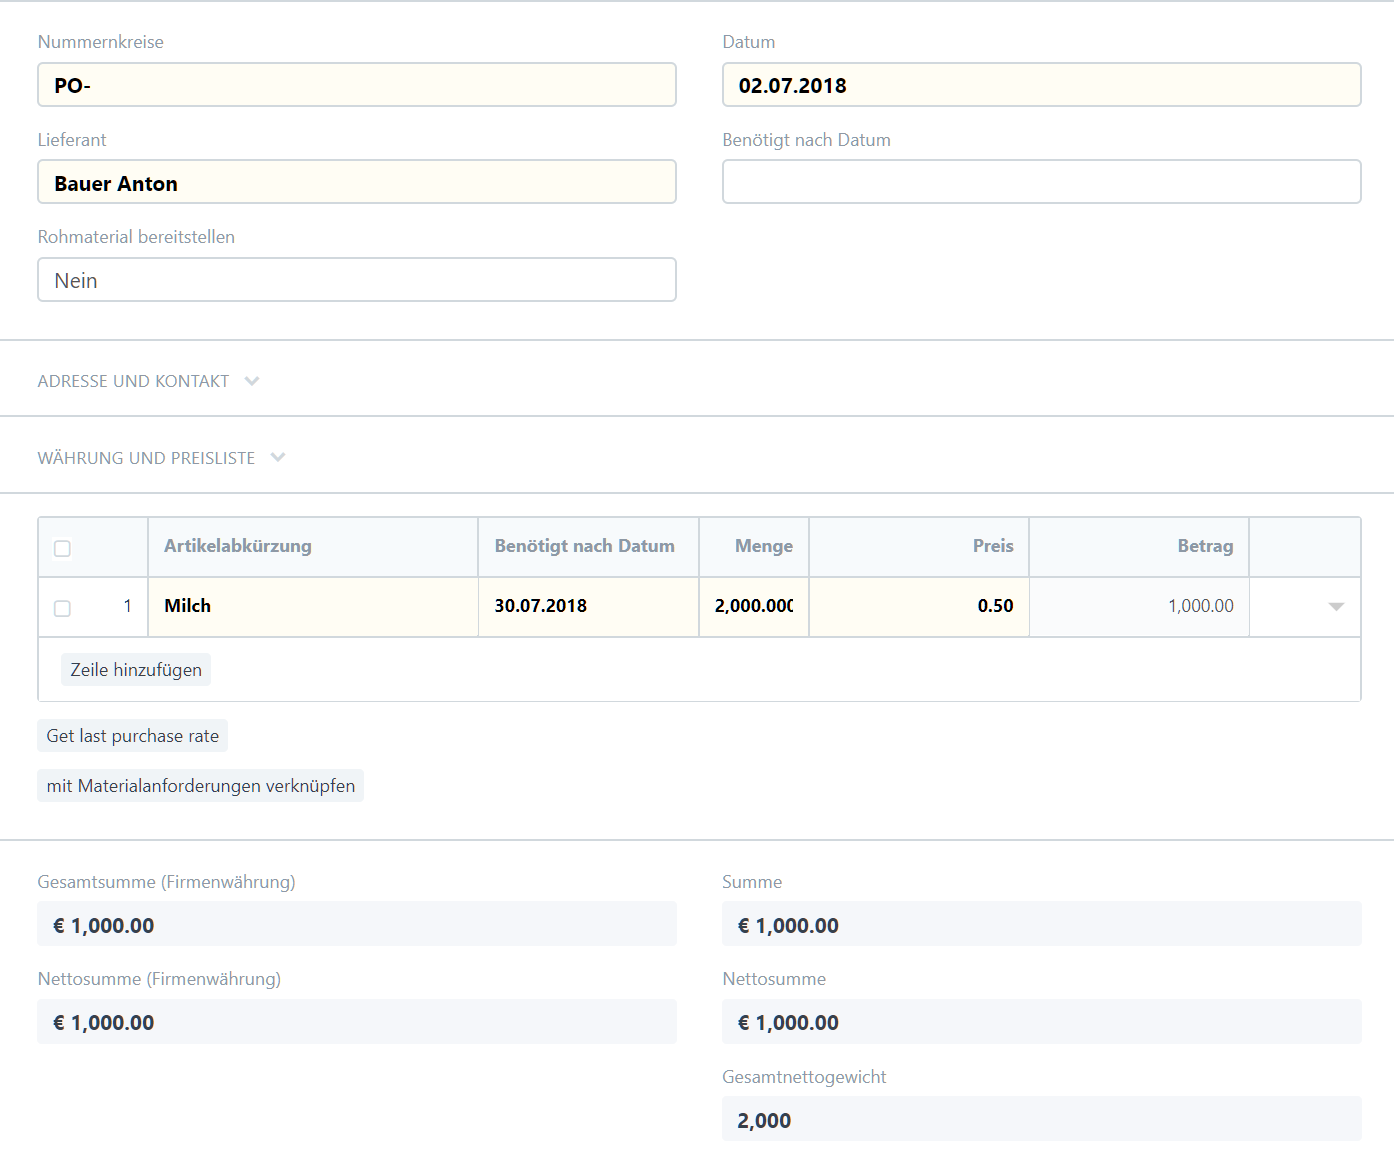
\includegraphics[width=\textwidth]{Bilder/Lieferantenauftrag.PNG}
  \caption{Anlegen eines neuen Lieferantenauftrages}
  \label{fig:liefAuftrag}
\end{figure}
\begin{figure}[H]
  \centering
  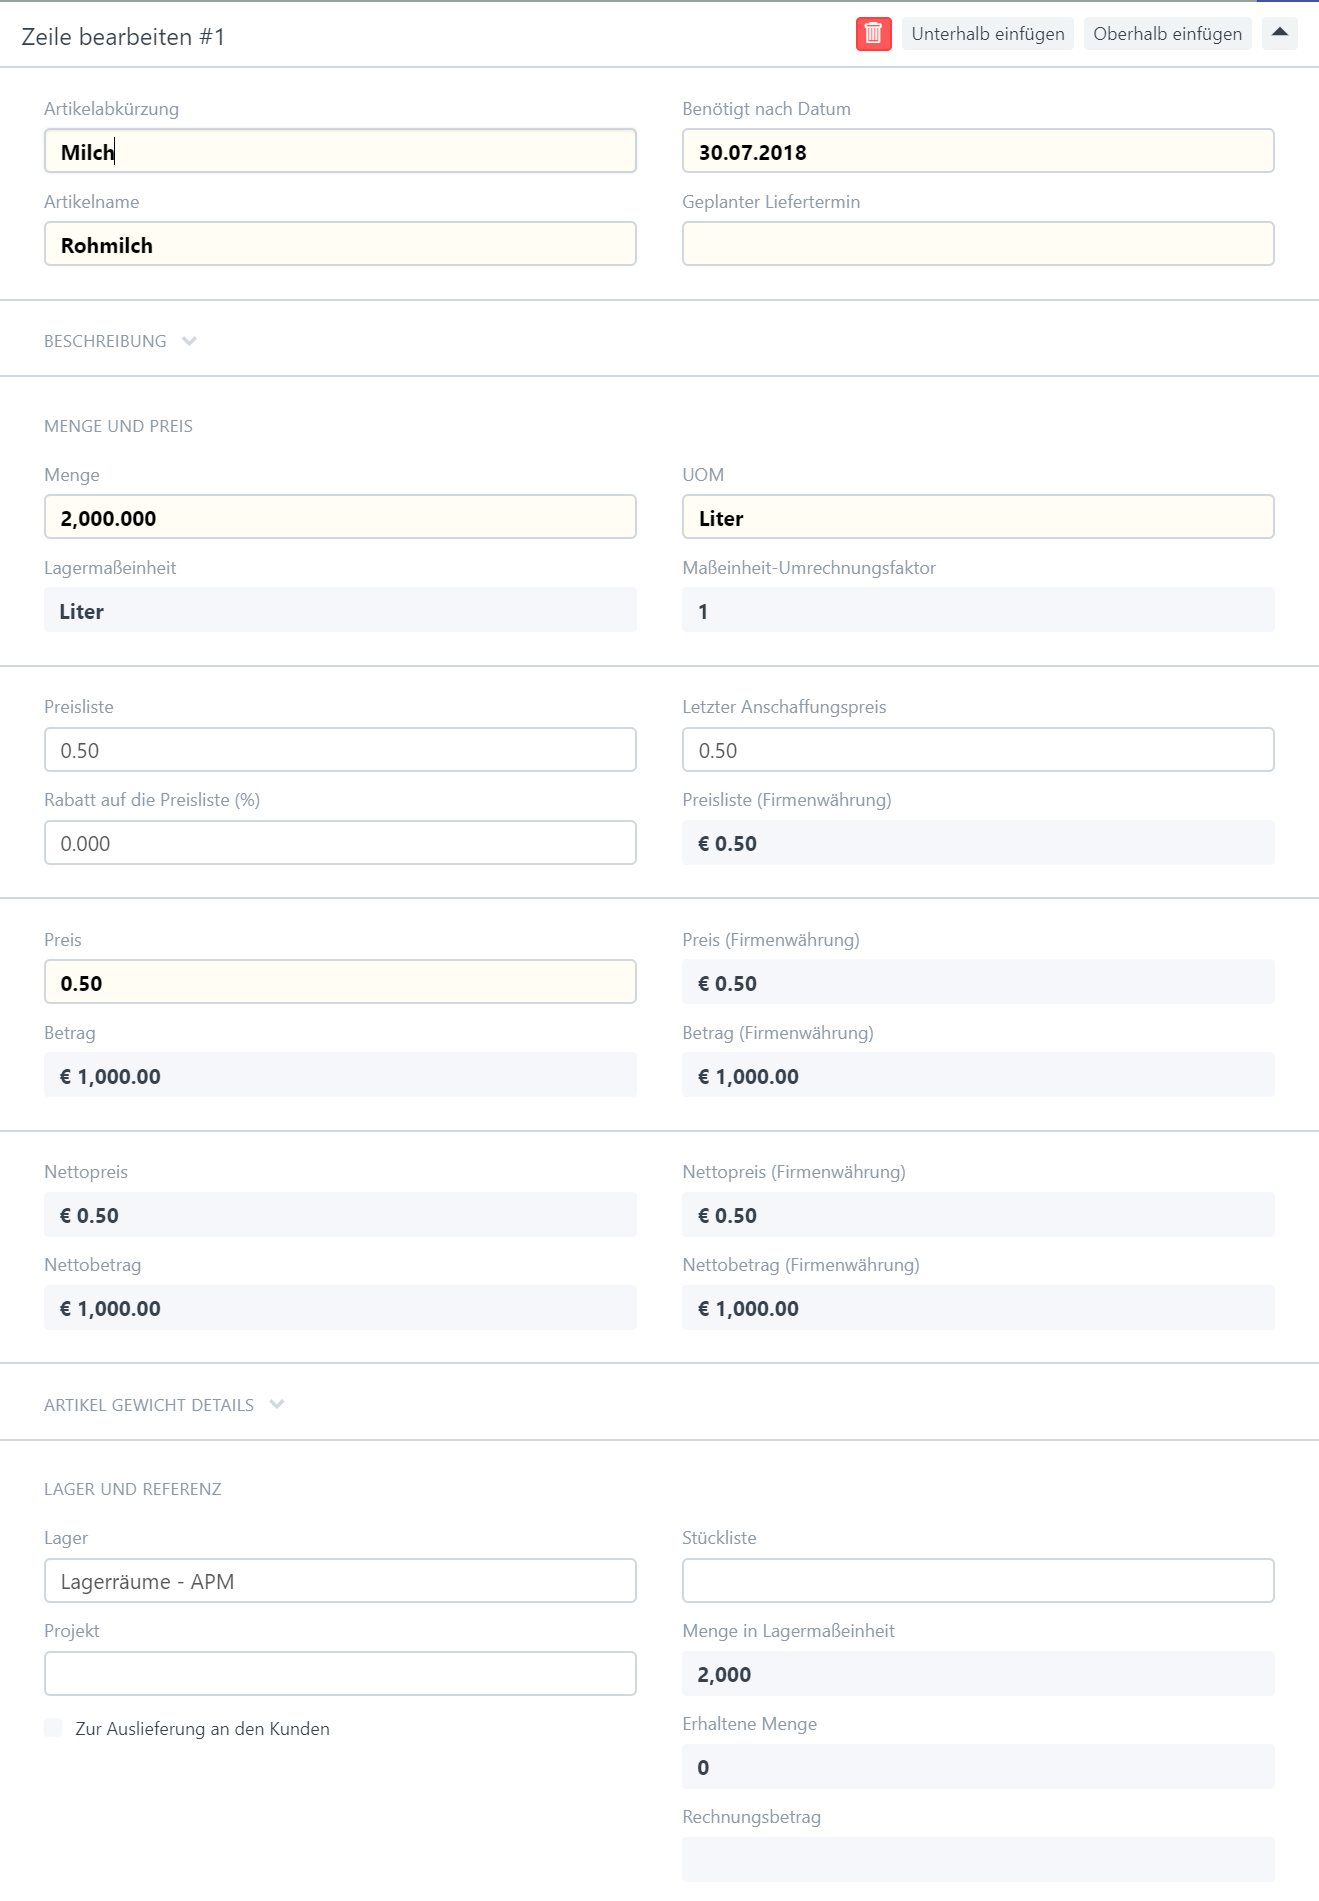
\includegraphics[width=\textwidth]{Bilder/Lieferantenauftrag_Produktdetail.PNG}
  \caption{Detailansicht eines Artikels eines Lieferantenauftrags}
  \label{fig:auftrDetail}
\end{figure}
\begin{figure}[H]
  \centering
  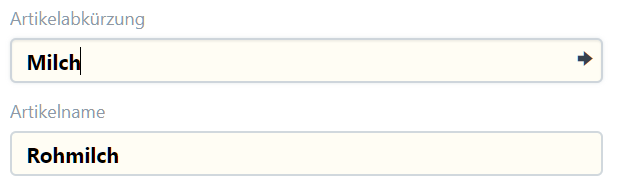
\includegraphics[width=\textwidth]{Bilder/Milch_Link.PNG}
  \caption{Verlinkung des Artikels Milch}
  \label{fig:verlArtikel}
\end{figure}
\begin{figure}[H]
  \centering
  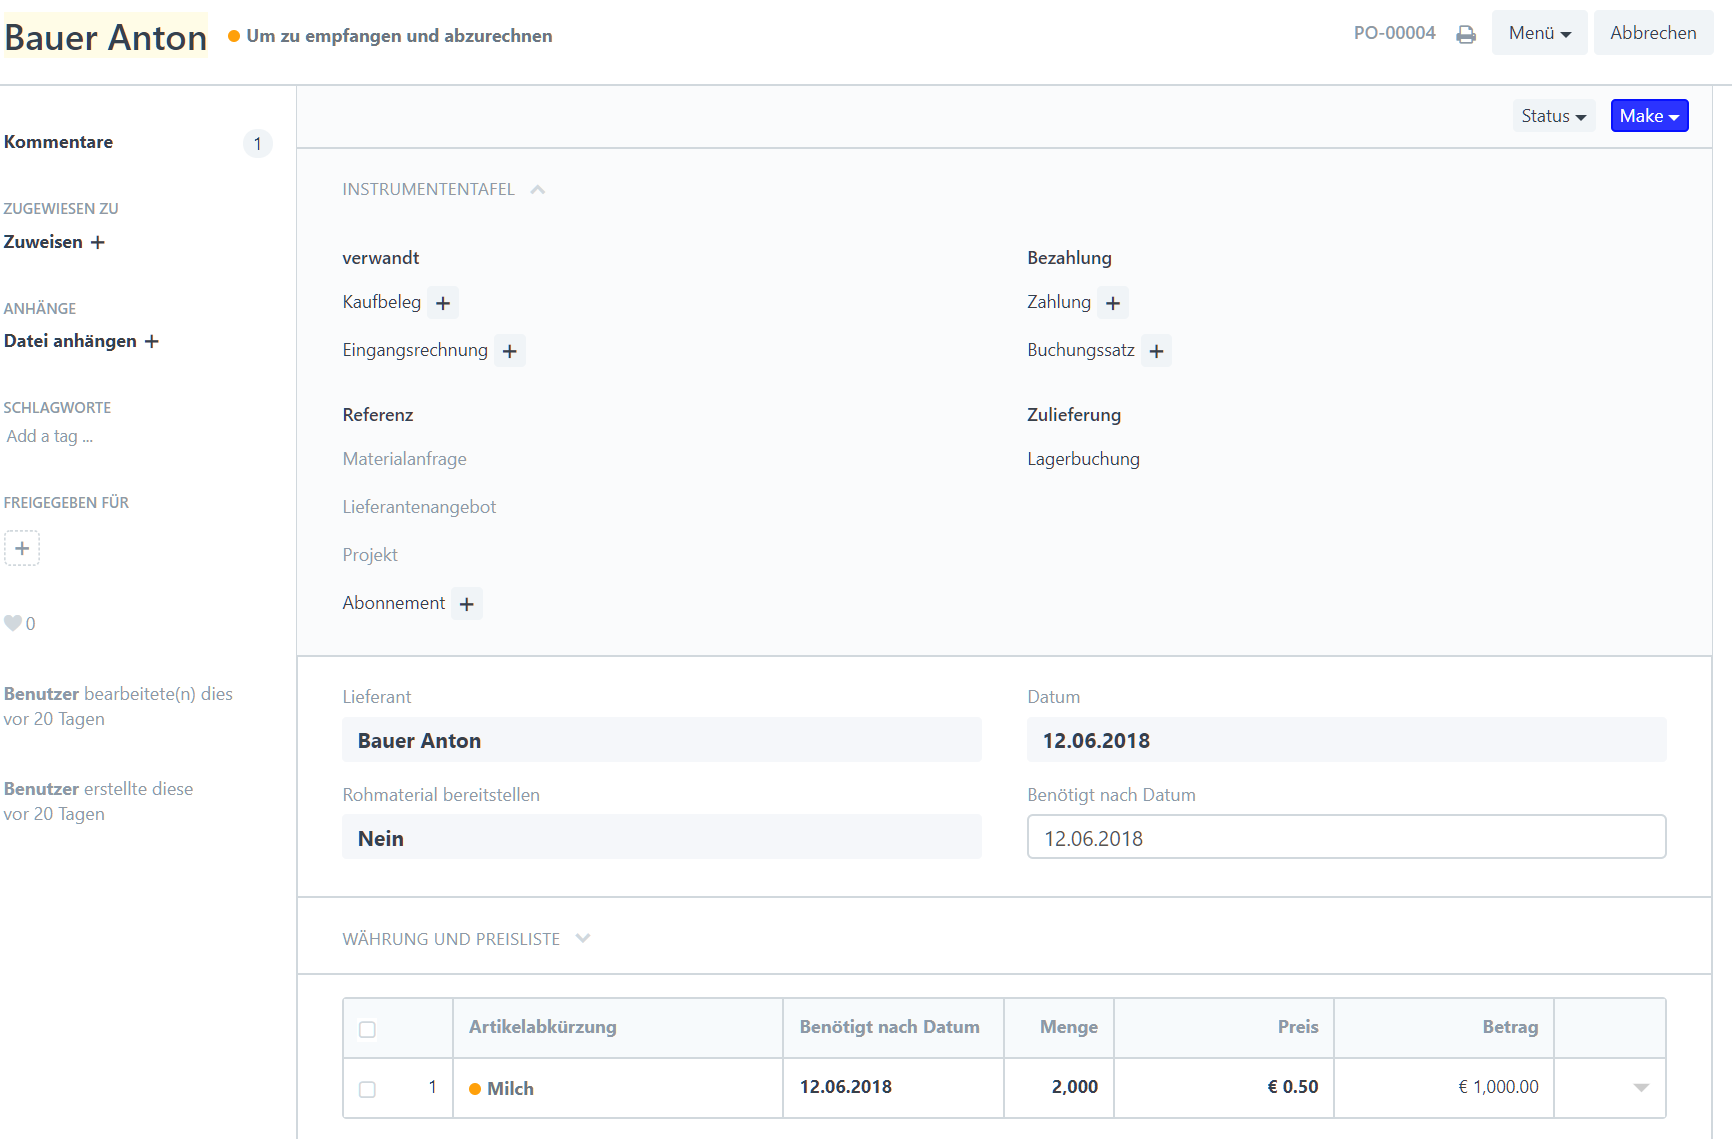
\includegraphics[width=\textwidth]{Bilder/Uebersicht_Lieferantenauftrag.PNG}
  \caption{Übersicht Lieferantenauftrag}
  \label{fig:auftrUebersicht}
\end{figure}
\begin{figure}[H]
  \centering
  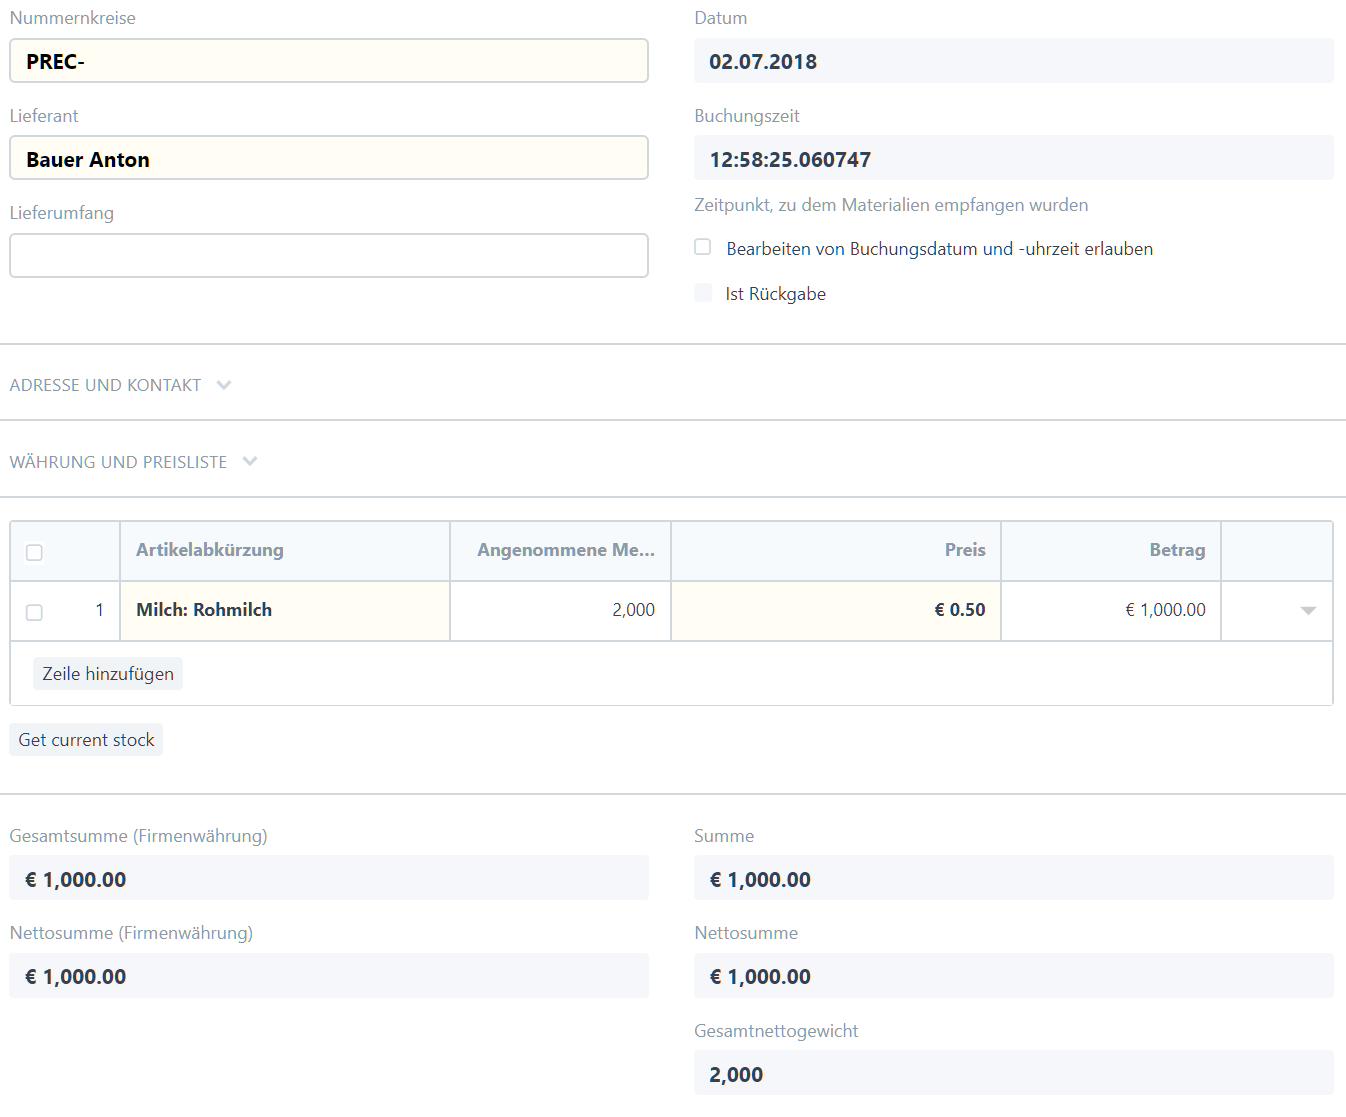
\includegraphics[width=\textwidth]{Bilder/Kaufbeleg.PNG}
  \caption{Kaufbeleg}
  \label{fig:kaufbeleg}
\end{figure}
\begin{figure}[H]
  \centering
  
\includegraphics[width=\textwidth]{Bilder/Mitteilung_Qualitaetspruefung.PNG}
  \caption{Mitteilung für eine erforderliche Qualitätsprüfung}
  \label{fig:mittQual}
\end{figure}
\begin{figure}[H]
  \centering
  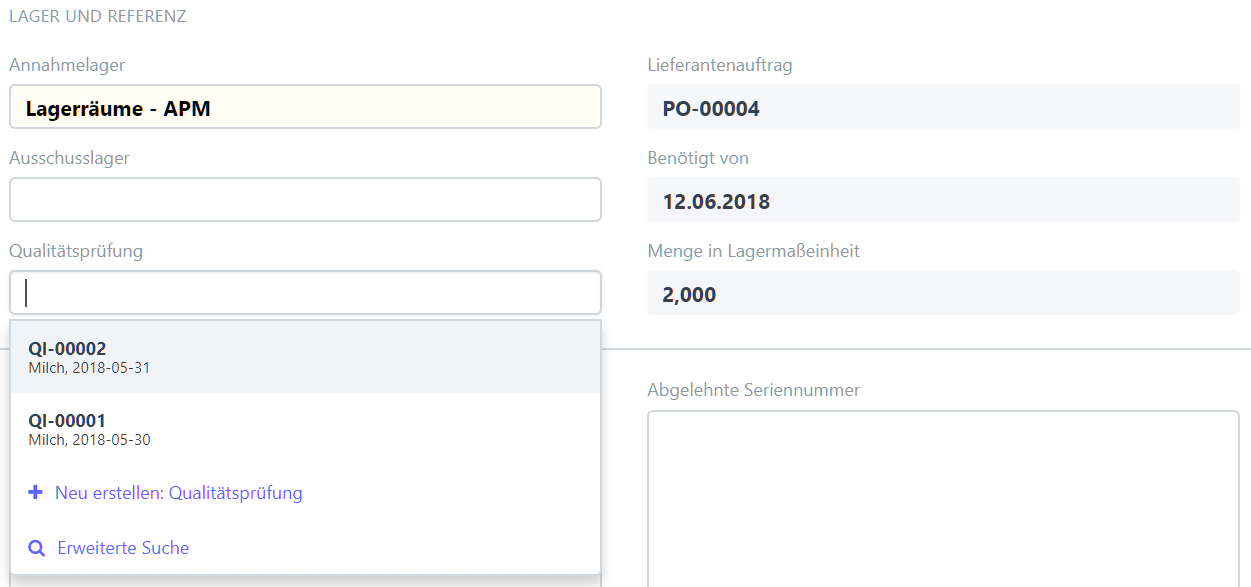
\includegraphics[width=\textwidth]{Bilder/Qualitaetskontrolle_auswaehlen.PNG}
  \caption{Auswahlmöglichkeiten bei der Qualitätsprüfung}
  \label{fig:auswQual}
\end{figure}
\begin{figure}[H]
  \centering
  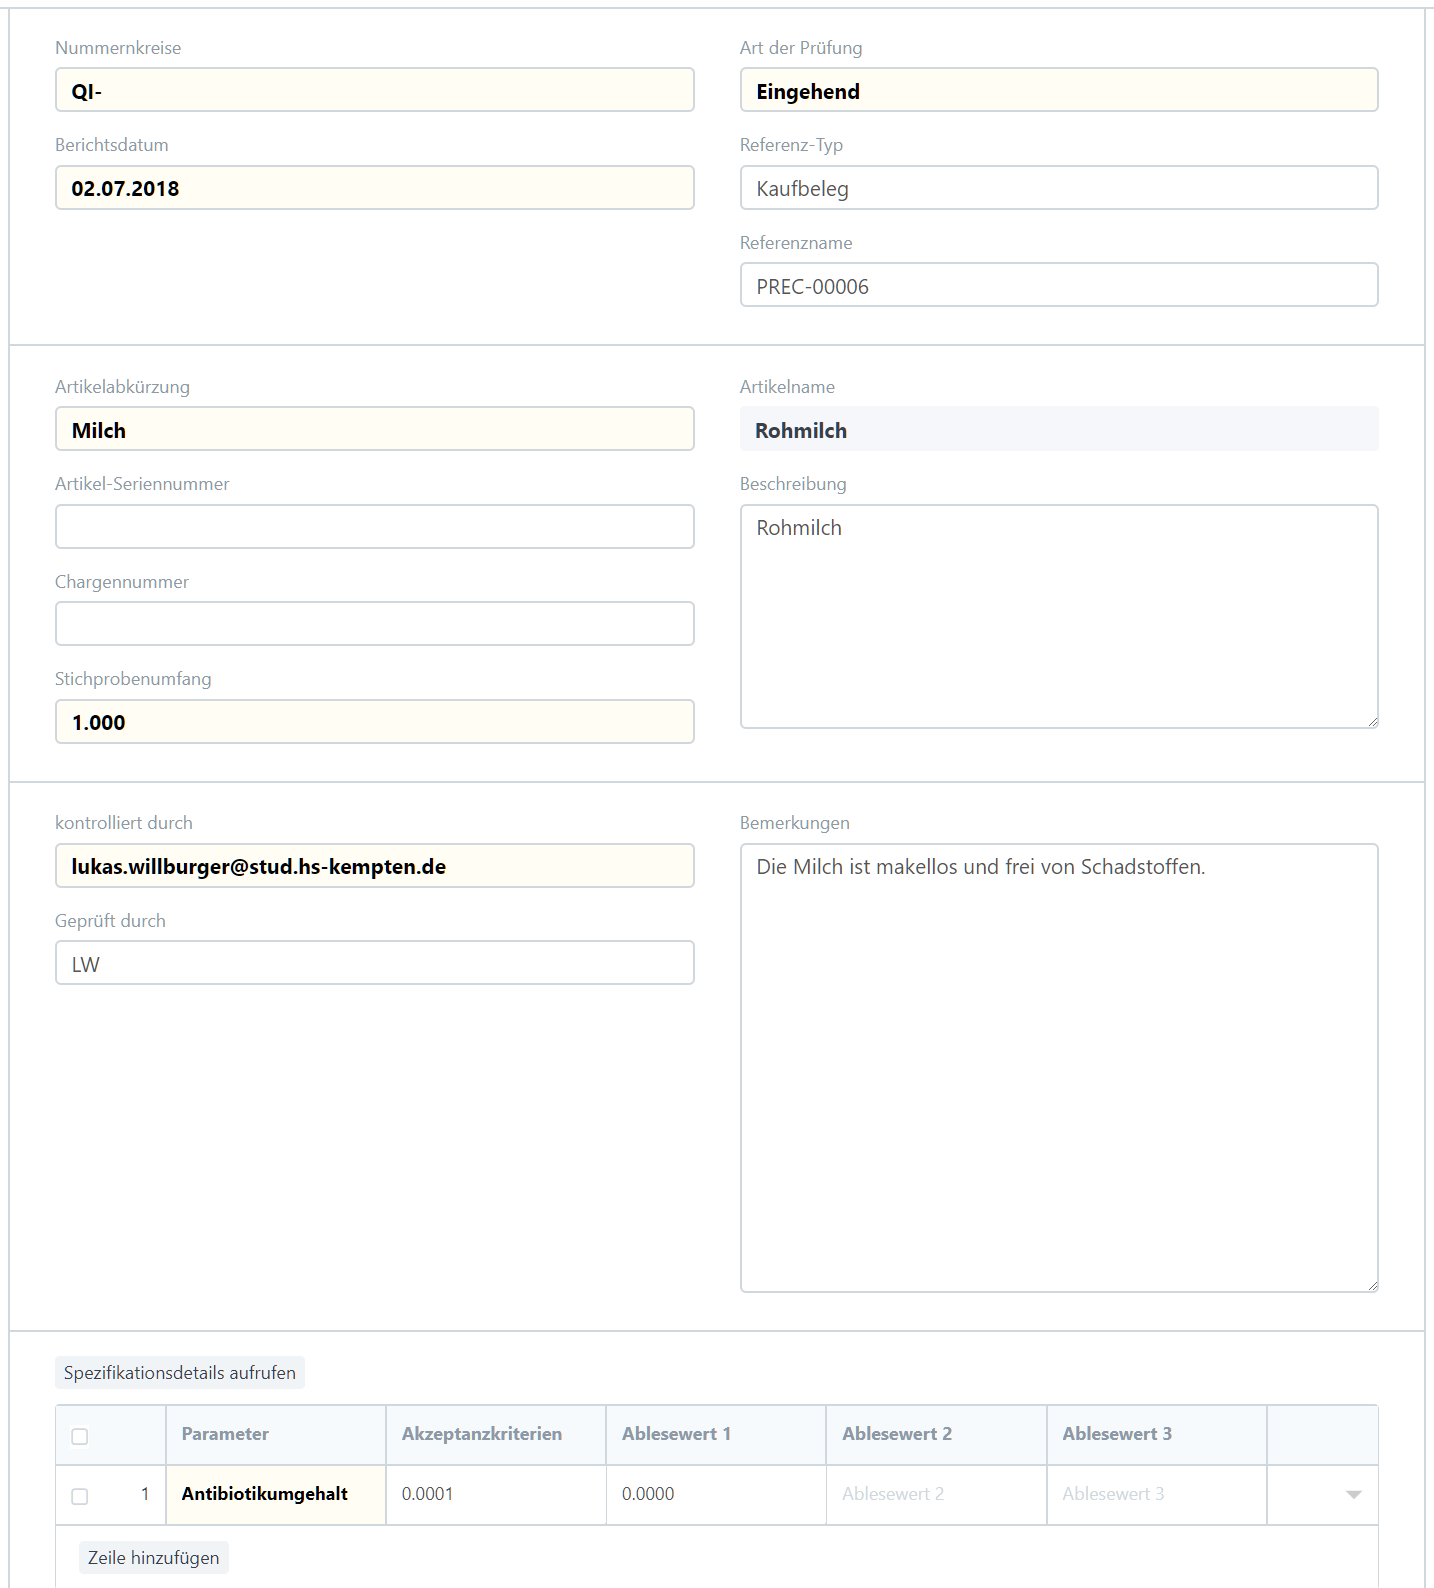
\includegraphics[width=\textwidth]{Bilder/Qualitaetspruefung.PNG}
  \caption{Übersicht der Qualitätsprüfung}
  \label{fig:qualPruef}
\end{figure}
\begin{figure}[H]
  \centering
  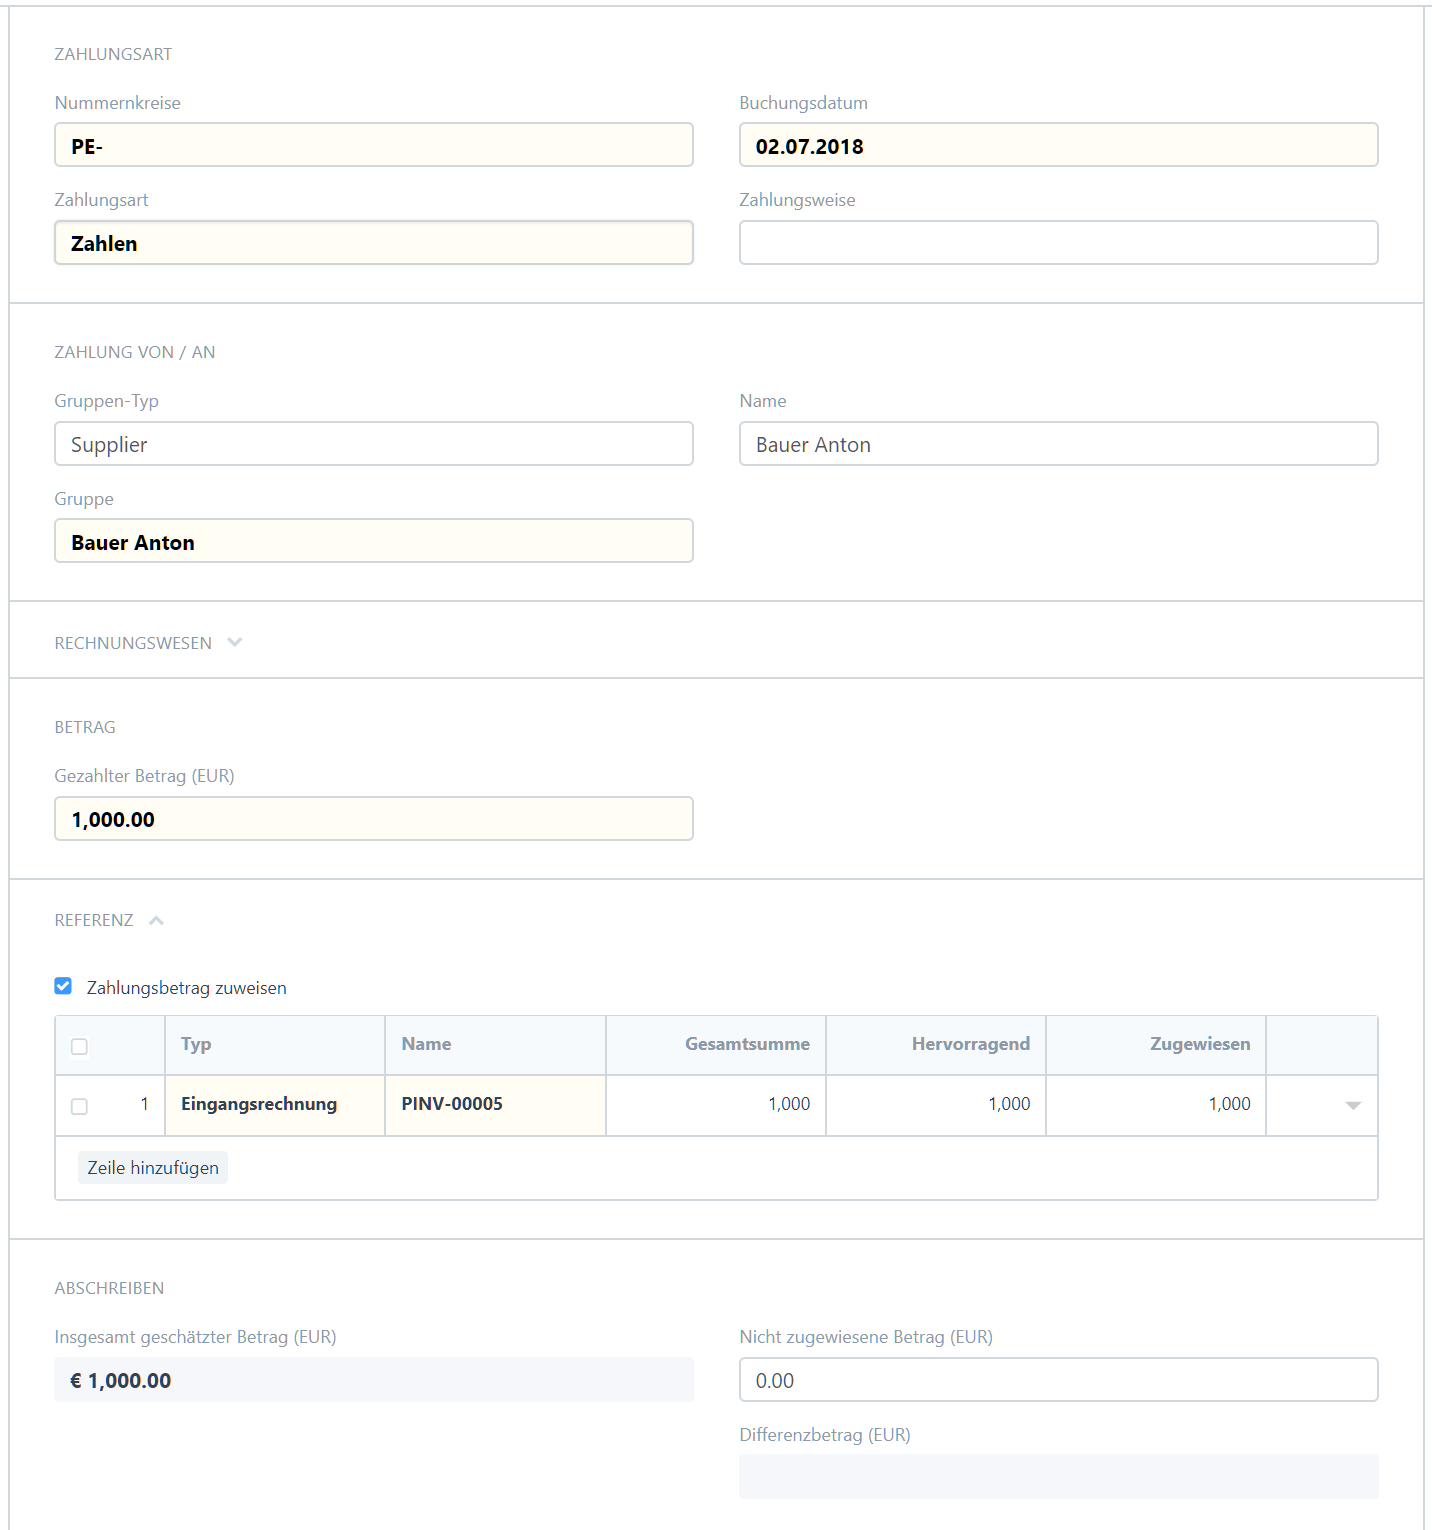
\includegraphics[width=\textwidth]{Bilder/Zahlung.PNG}
  \caption{Zahlung mit Rechnungsverknüpfung}
  \label{fig:zahlung}
\end{figure}
\begin{figure}[H]
  \centering
  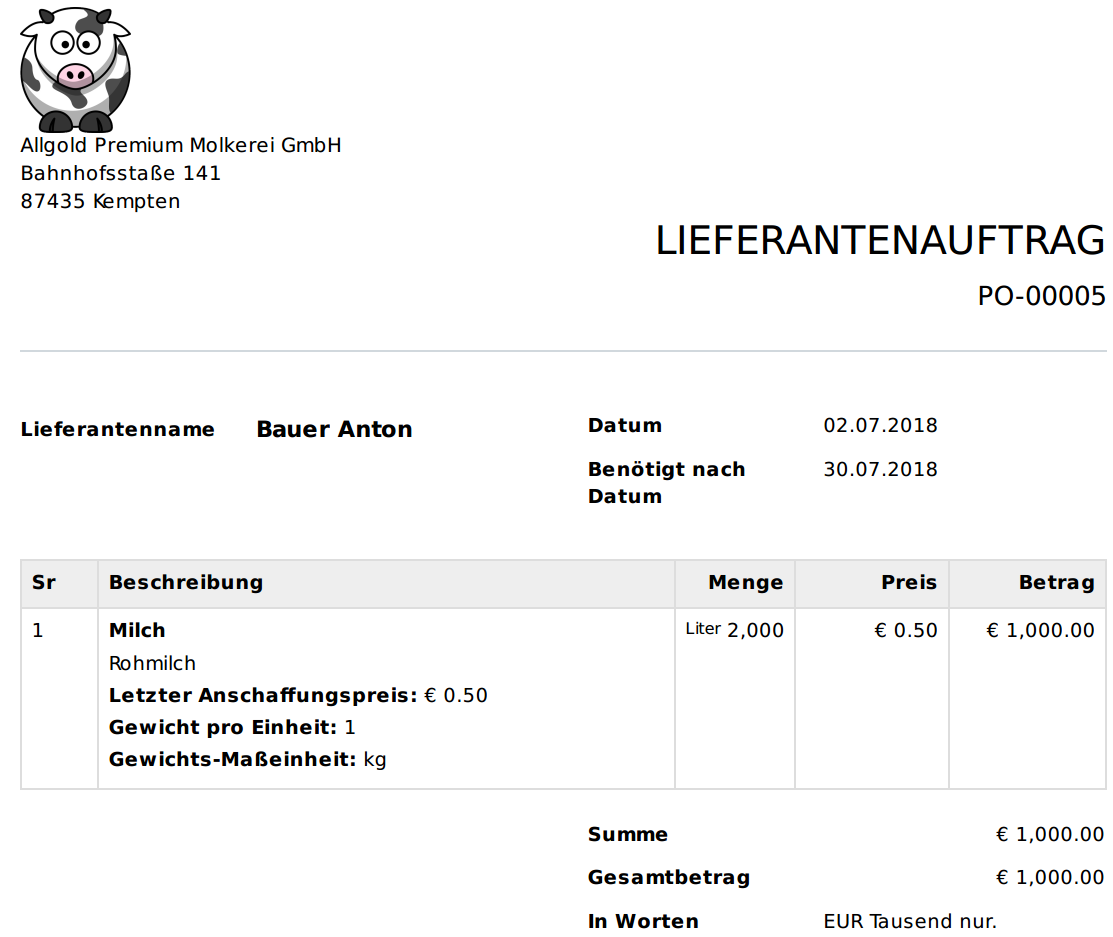
\includegraphics[width=\textwidth]{Bilder/Auftrag_Mail.PNG}
  \caption{Lieferantenauftrag als PDF}
  \label{fig:auftrPdf}
\end{figure}
\begin{figure}[H]
  \centering
  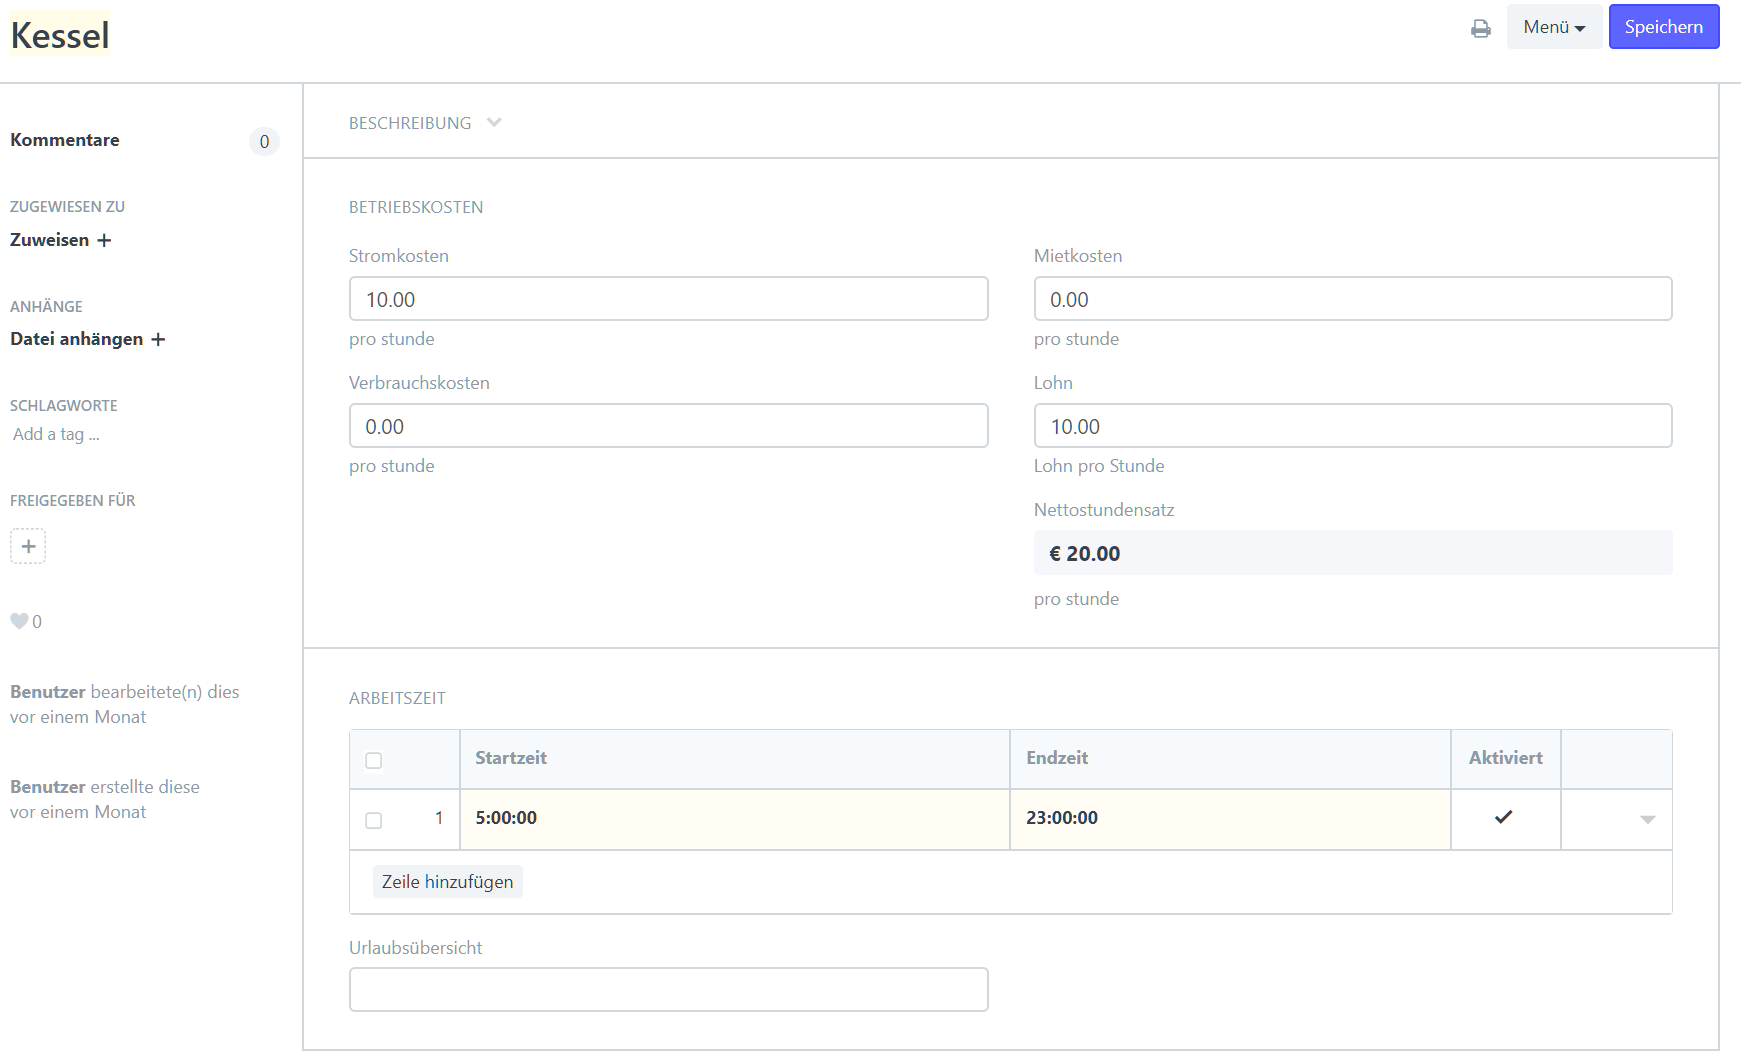
\includegraphics[width=\textwidth]{Bilder/Arbeitsplatz.PNG}
  \caption{Arbeitsplatz \glqq Kessel\grqq}
  \label{fig:arbPlatz}
\end{figure}
\begin{figure}[H]
  \centering
  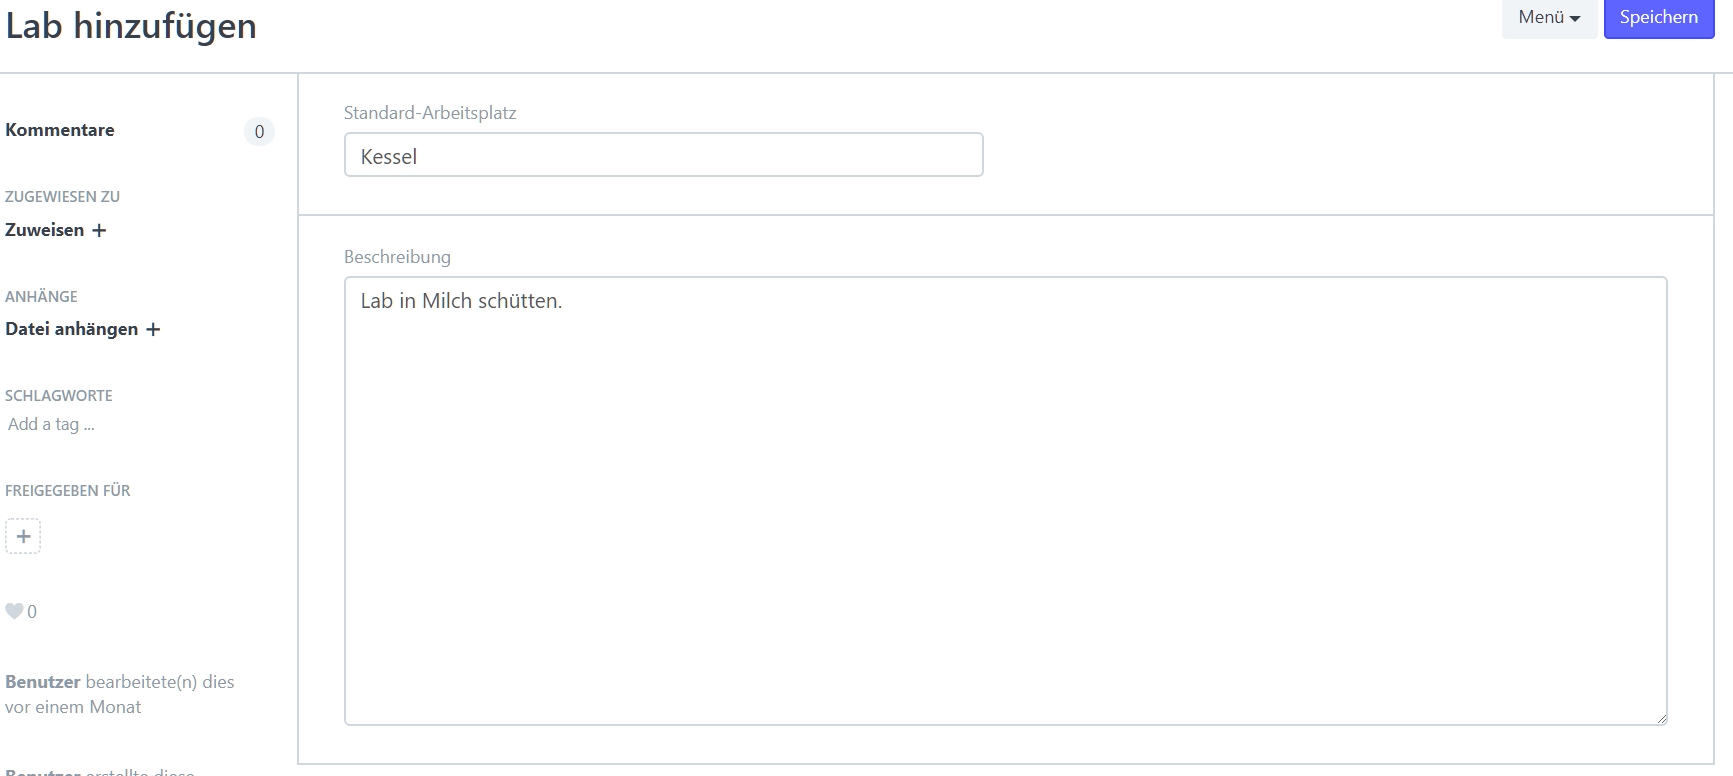
\includegraphics[width=\textwidth]{Bilder/Arbeitsgang.PNG}
  \caption{Arbeitsgang \glqq Lab hinzufügen\grqq}
  \label{fig:arbGang}
\end{figure}
\begin{figure}[H]
  \centering
  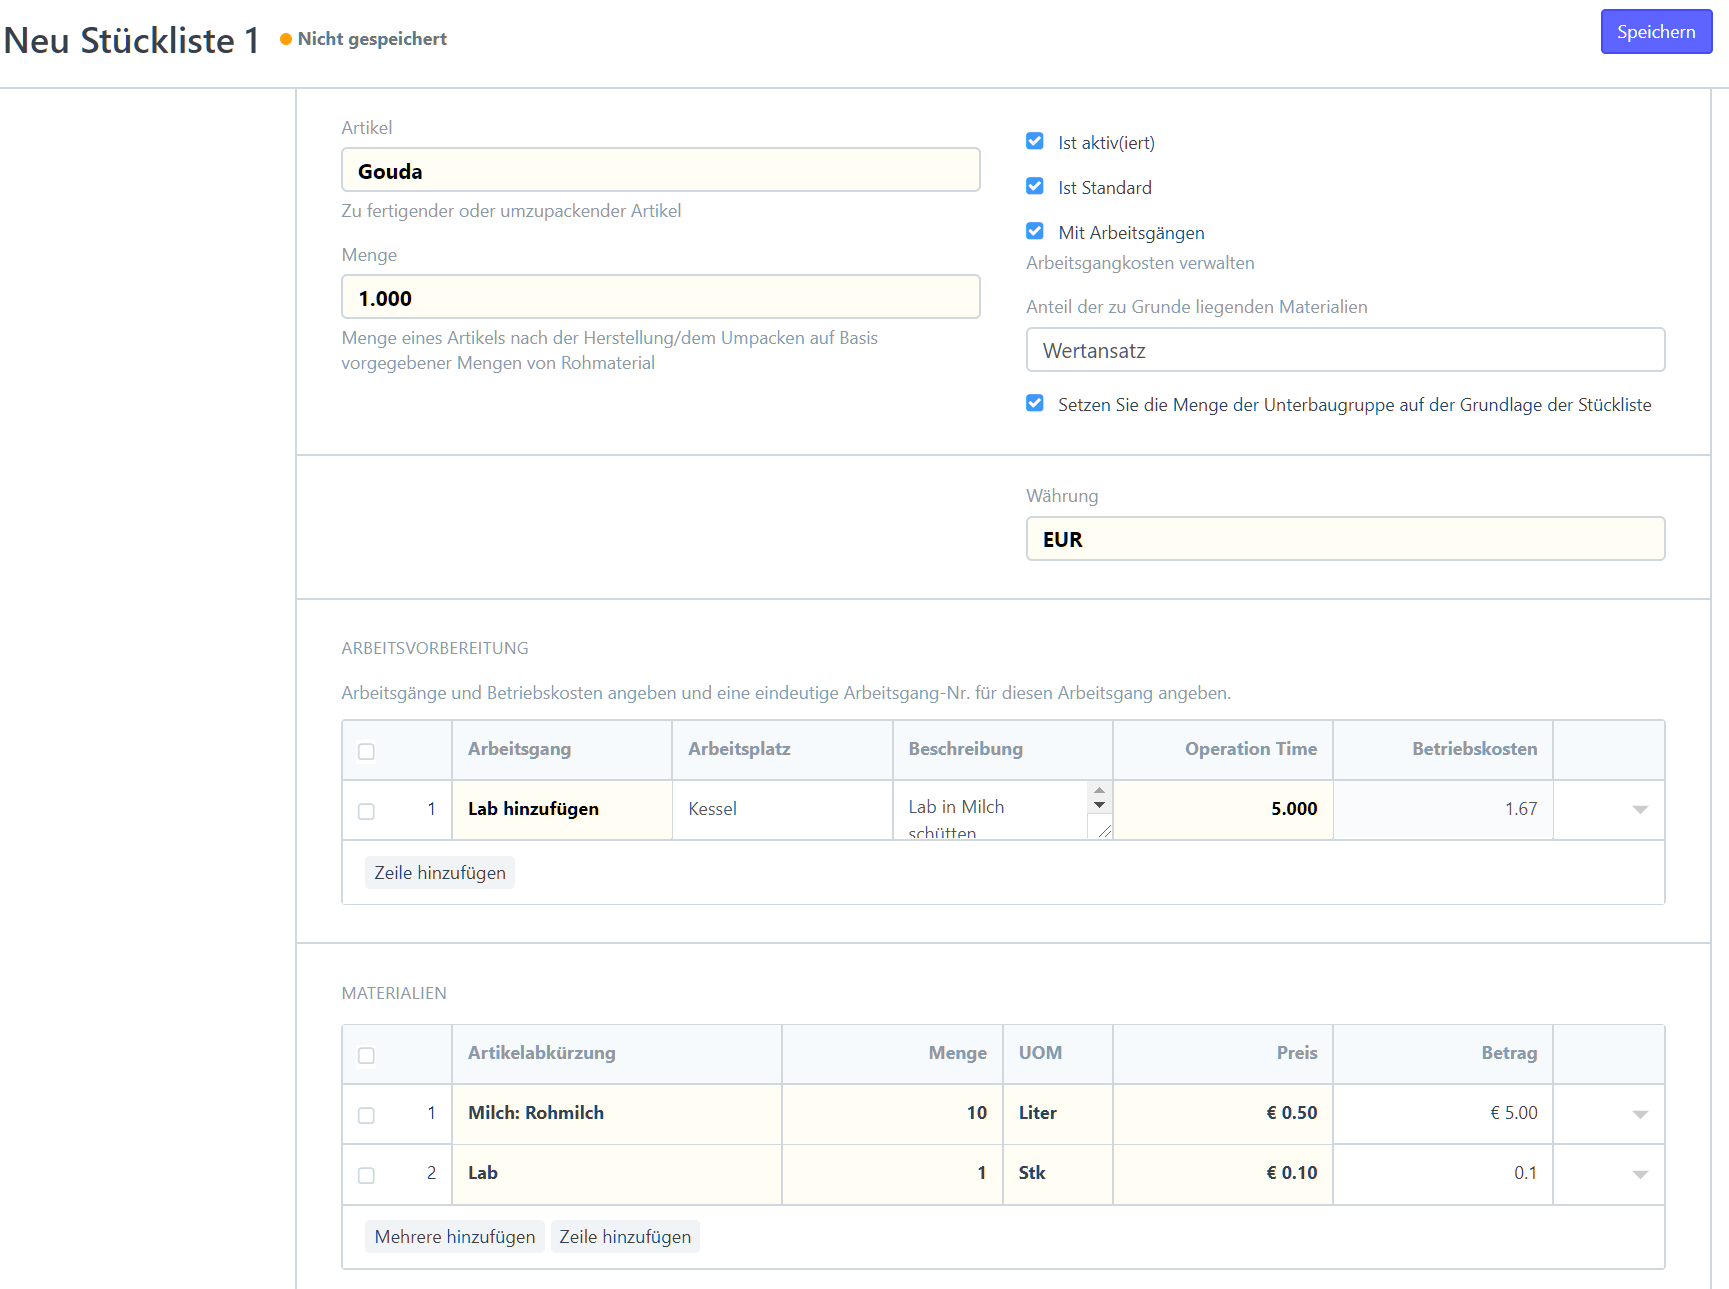
\includegraphics[width=\textwidth]{Bilder/Stueckliste.PNG}
  \caption{Stückliste für Gouda}
  \label{fig:stListe}
\end{figure}
\begin{figure}[H]
  \centering
  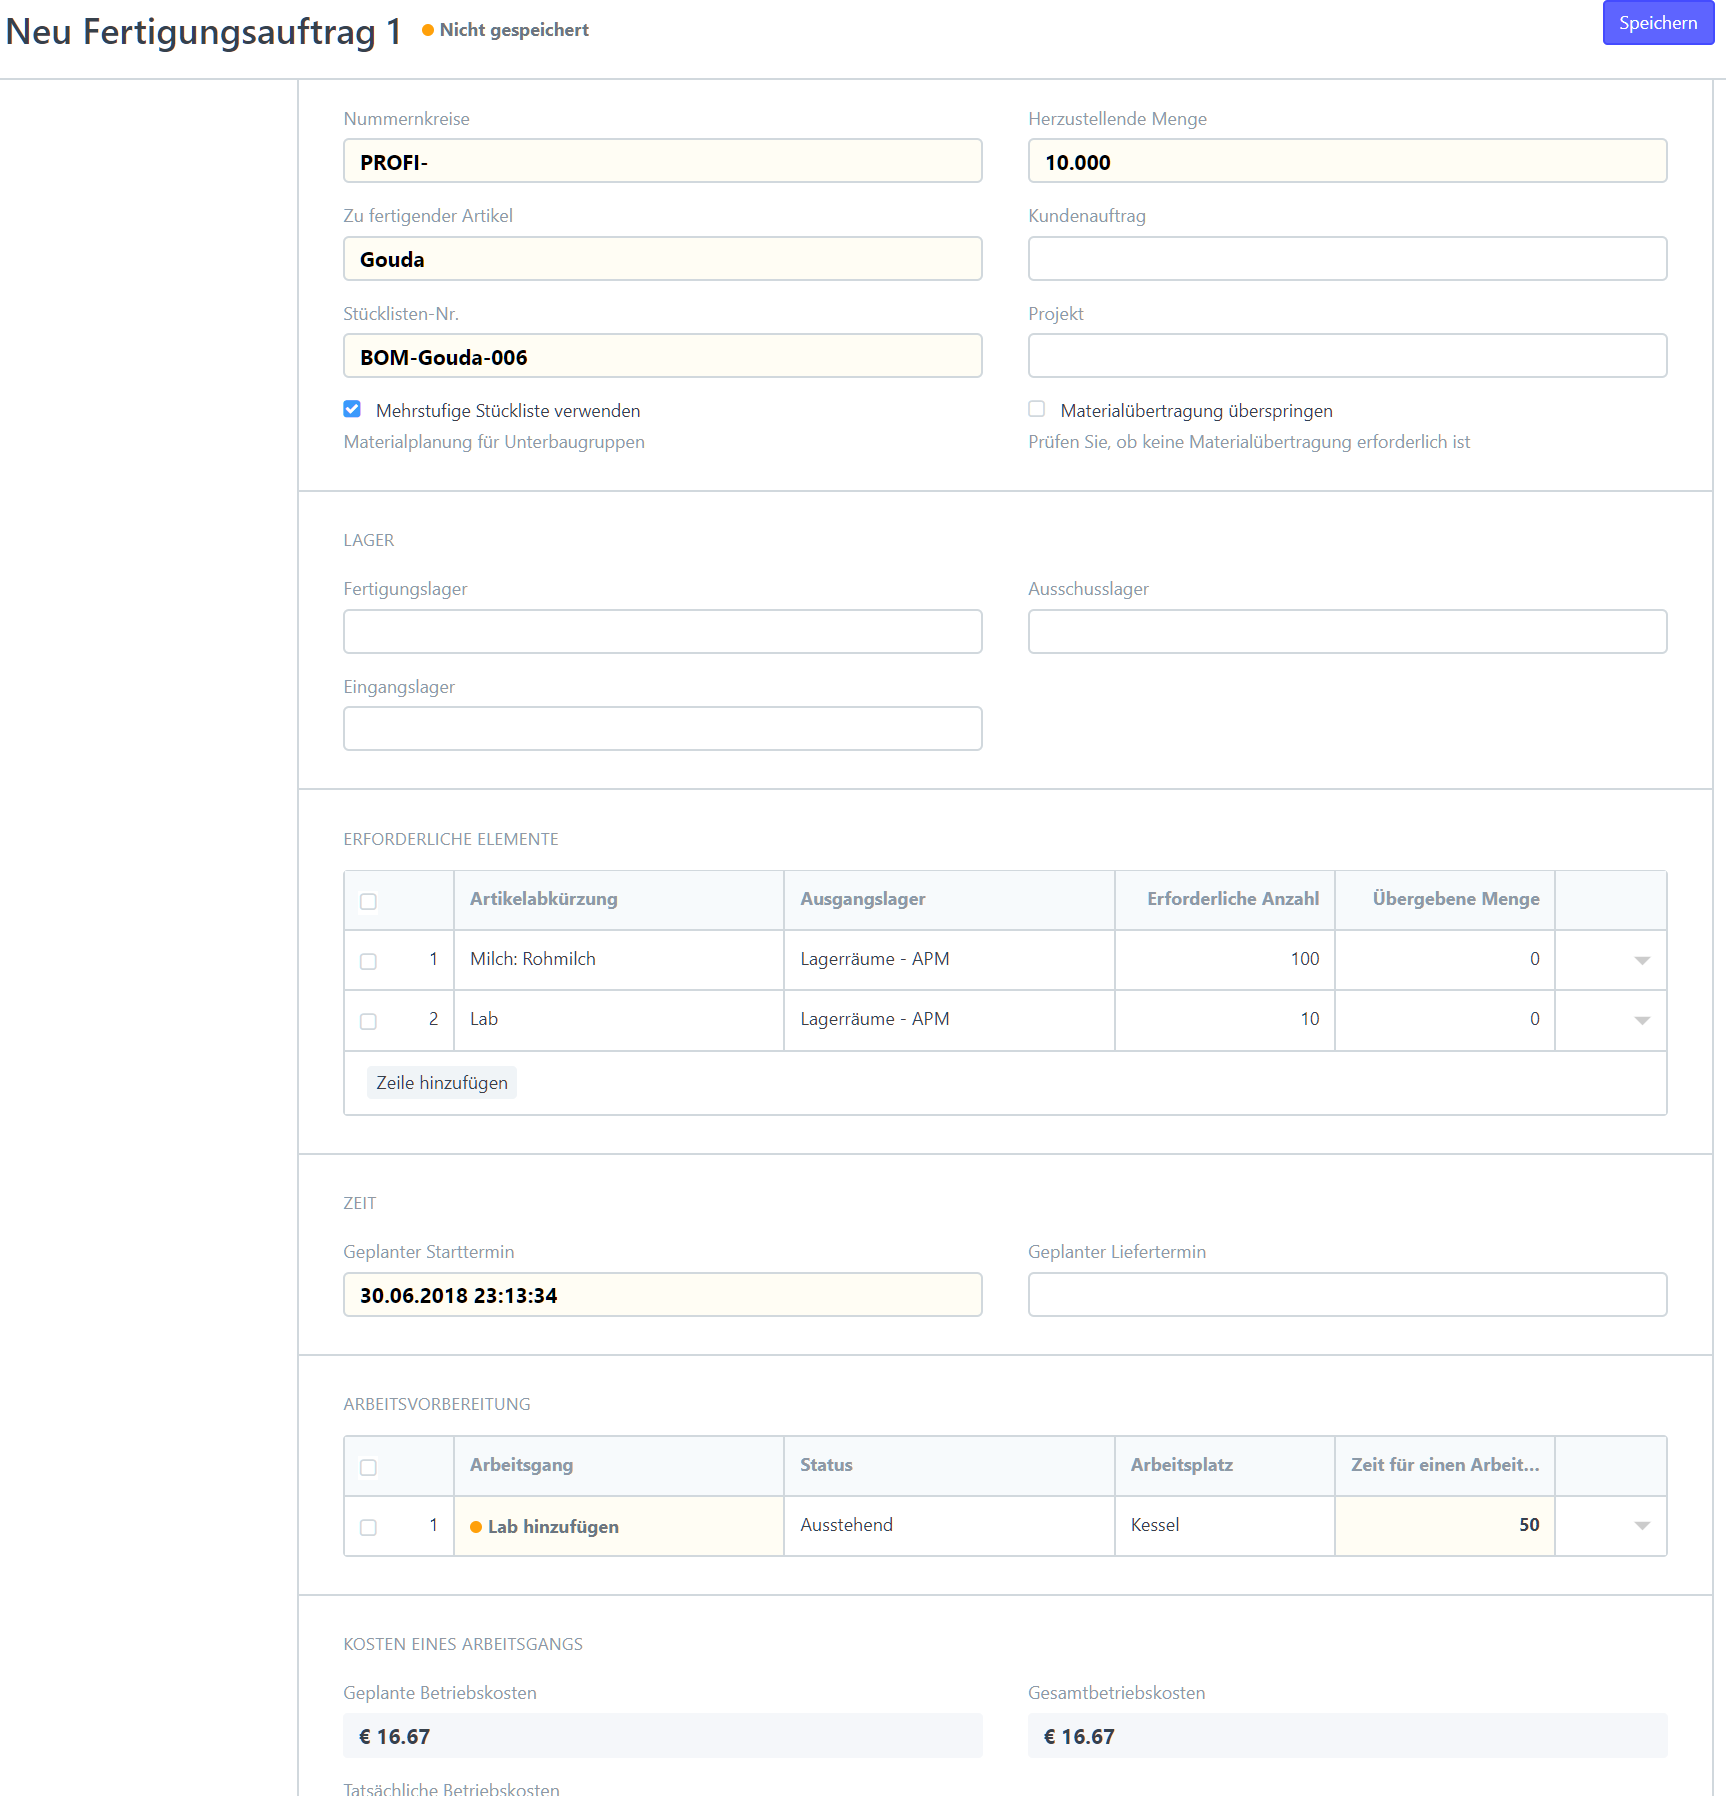
\includegraphics[width=\textwidth]{Bilder/Fertigungsauftrag.PNG}
  \caption{Fertigungsauftrag für Gouda}
  \label{fig:fertAuftr}
\end{figure}
\begin{figure}[H]
  \centering
  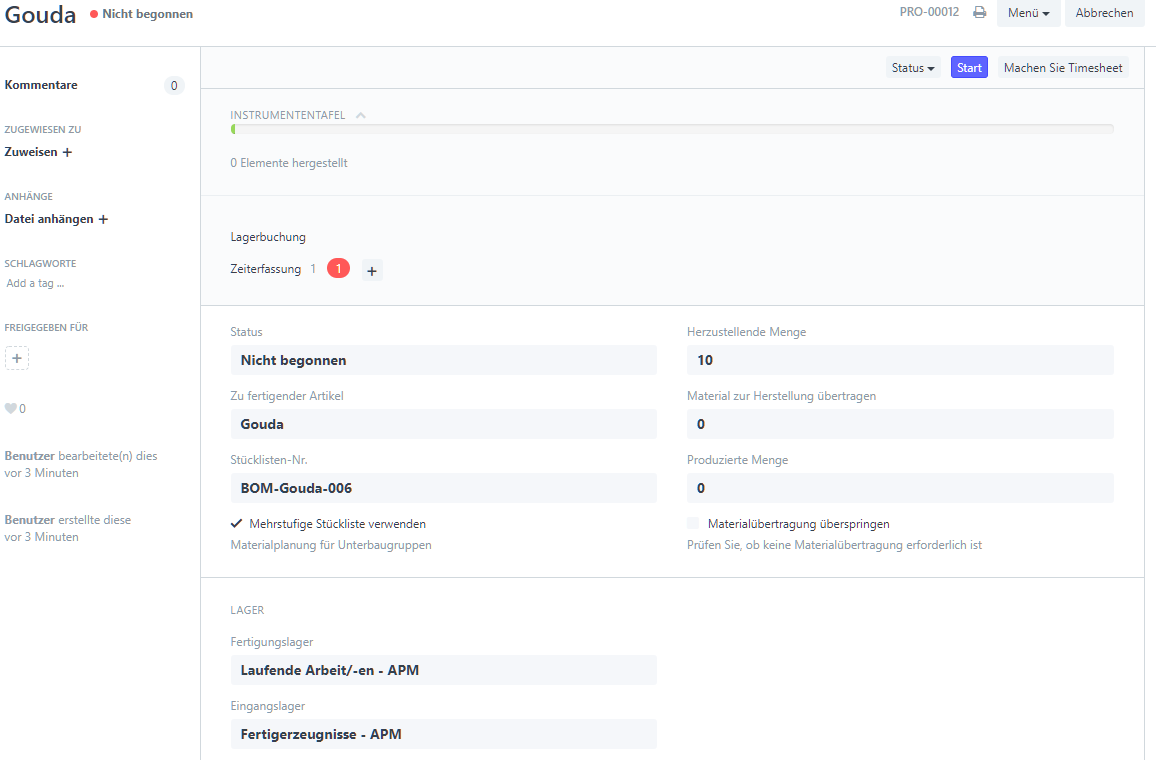
\includegraphics[width=\textwidth]{Bilder/Fertigungsauftrag_nicht_begonnen.PNG}
  \caption{Fertigungsauftrag (Herstellung noch nicht begonnen)}
  \label{fig:fertNichtBeg}
\end{figure}
\begin{figure}[H]
  \centering
  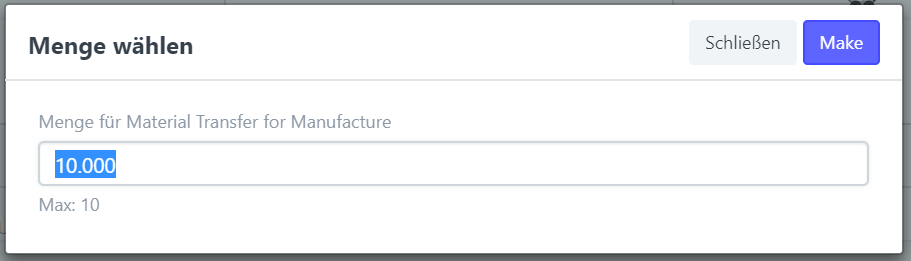
\includegraphics[width=\textwidth]{Bilder/Materialtransfer.PNG}
  \caption{Materialtransfer für die Herstellung}
  \label{fig:matTransfer}
\end{figure}
\begin{figure}[H]
  \centering
  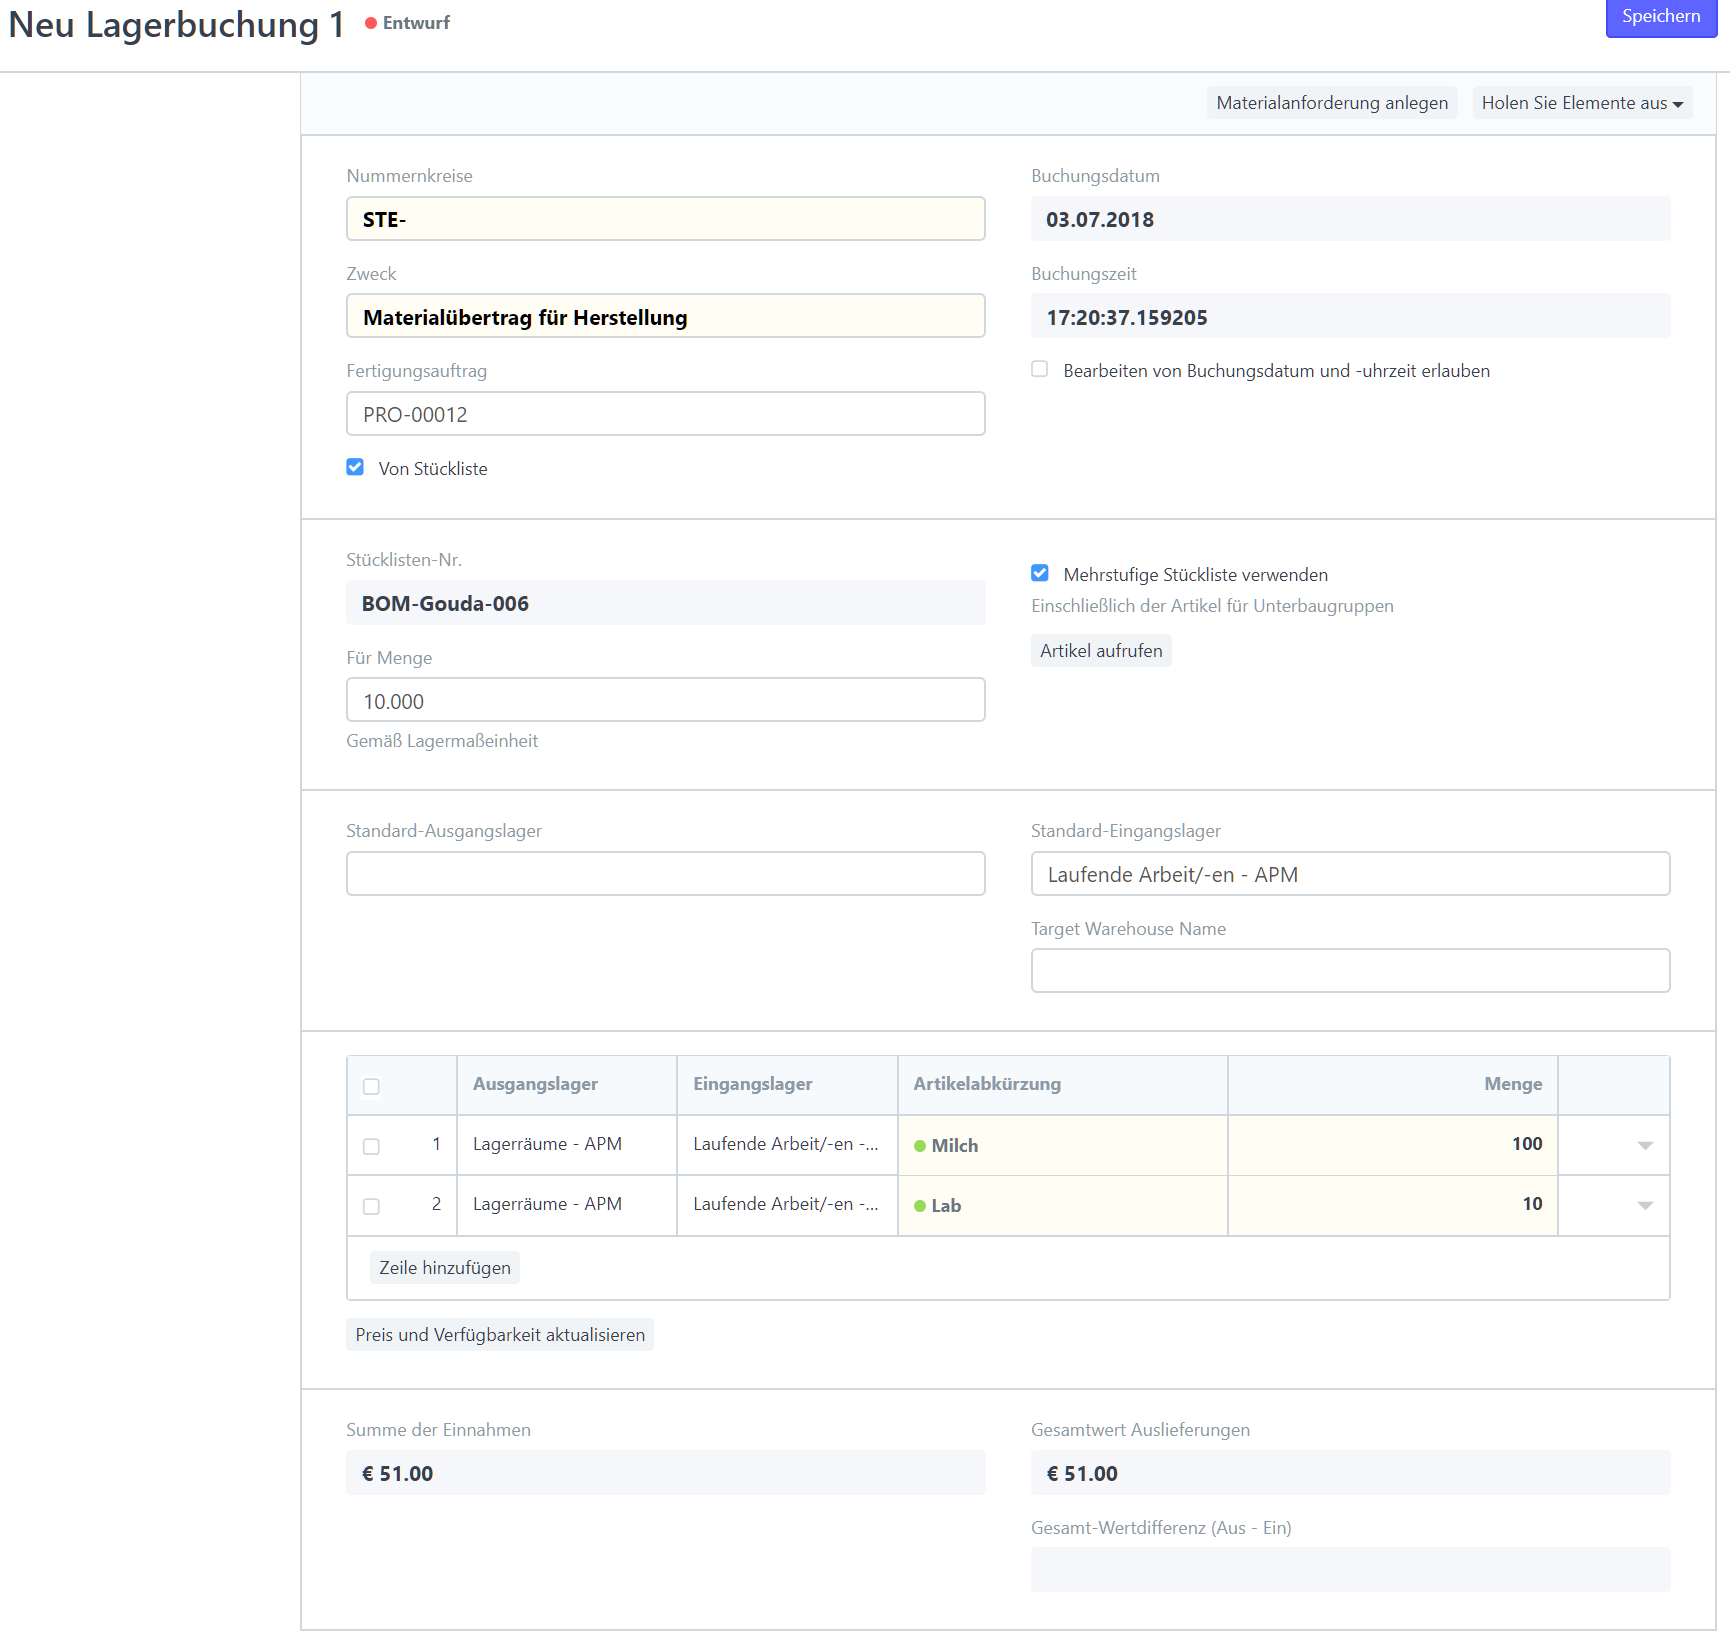
\includegraphics[width=\textwidth]{Bilder/Lagerbuchung.PNG}
  \caption{Lagerbuchung für die Herstellung}
  \label{fig:lagBuchung}
\end{figure}
\begin{figure}[H]
  \centering
  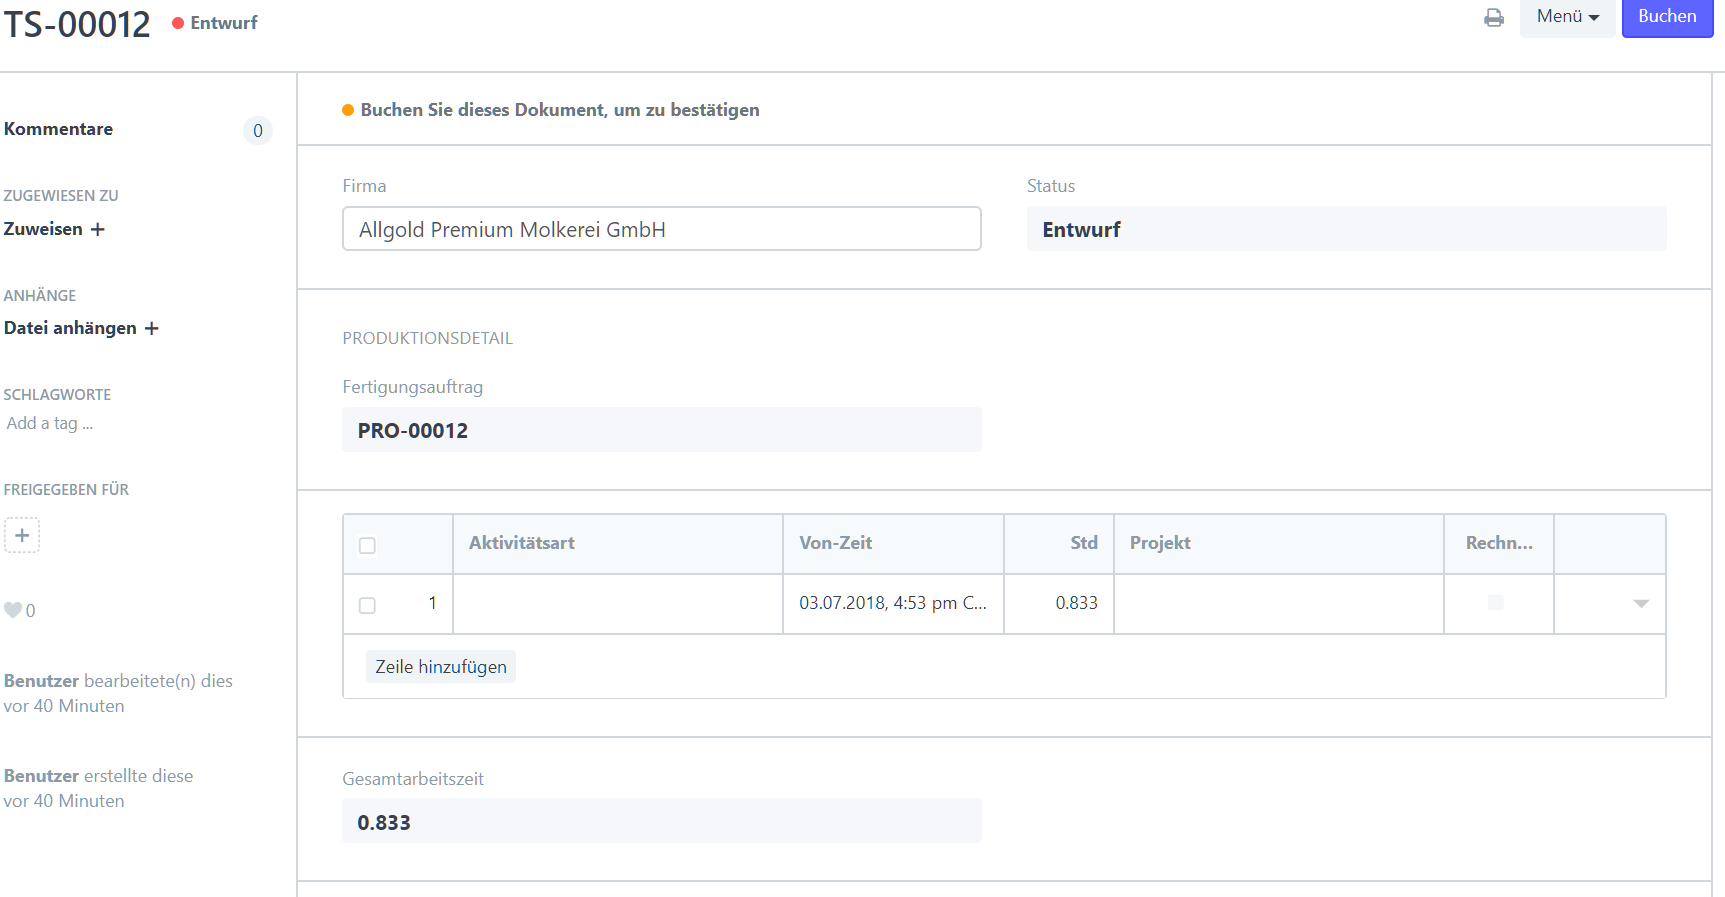
\includegraphics[width=\textwidth]{Bilder/Timesheet.PNG}
  \caption{Buchung der Zeiten}
  \label{fig:timeSheet}
\end{figure}
\begin{figure}[H]
  \centering
  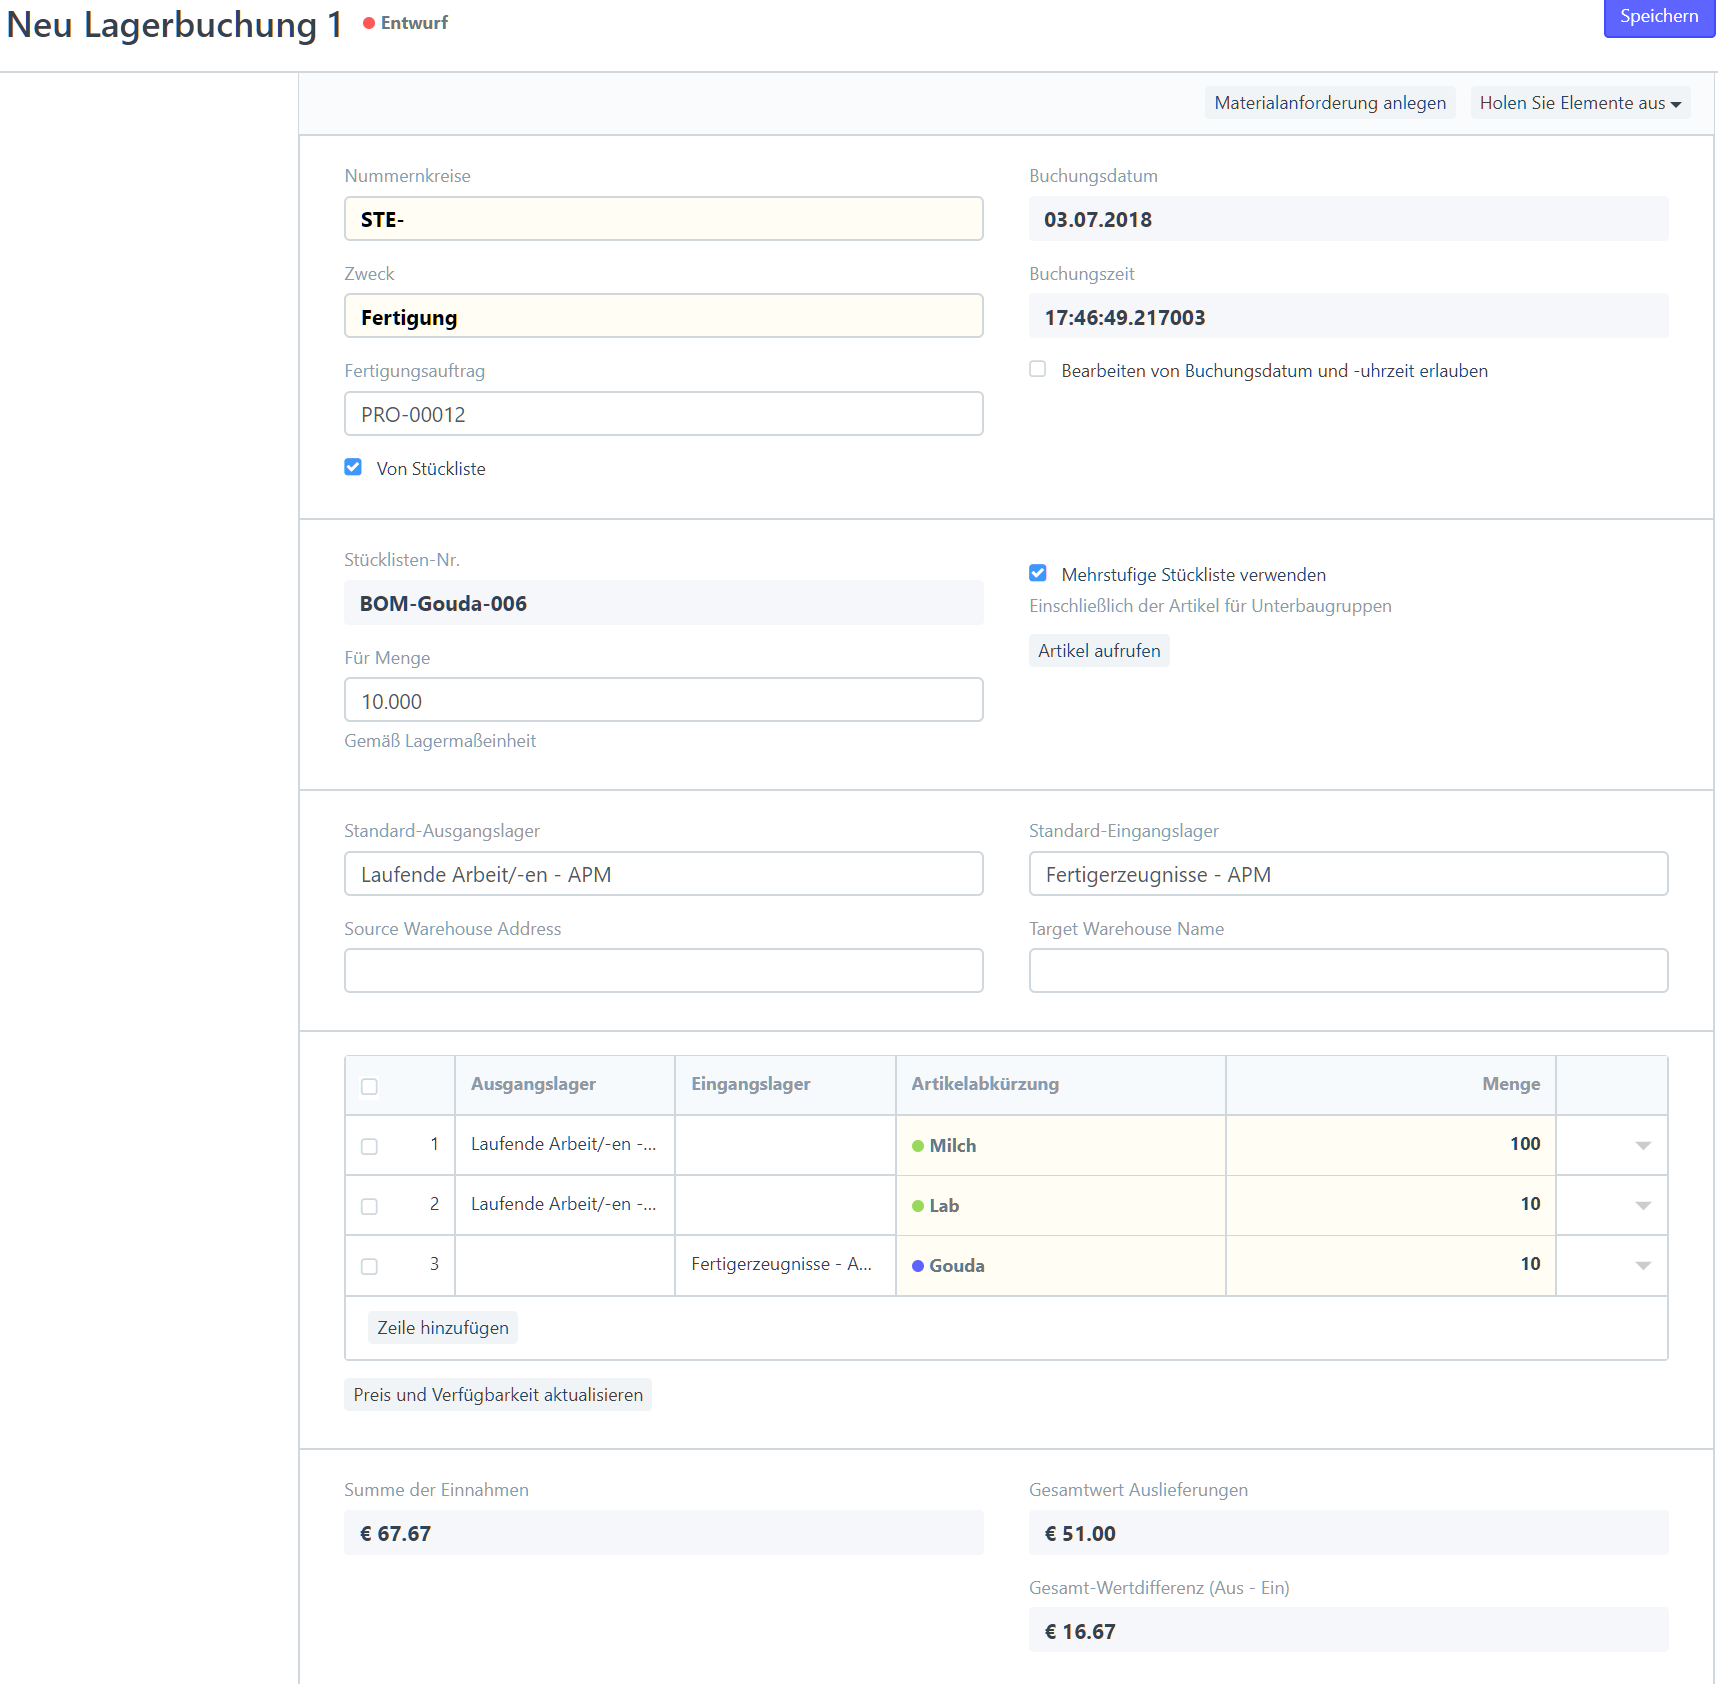
\includegraphics[width=\textwidth]{Bilder/Lagerbuchung2.PNG}
  \caption{Beendigung des Fertigungsauftrages}
  \label{fig:beenFertig}
\end{figure}
\begin{figure}[H]
  \centering
  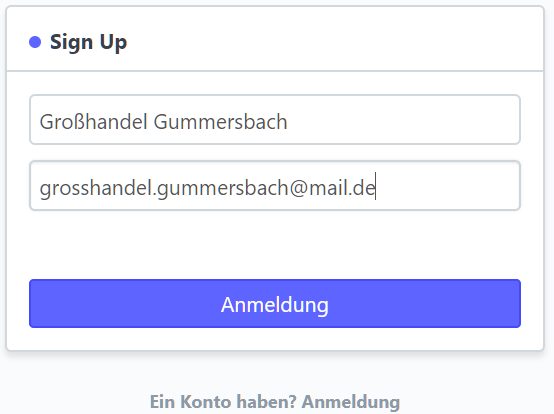
\includegraphics[width=\textwidth]{Bilder/Registrierung.PNG}
  \caption{Registrierung eines neuen Kunden}
  \label{fig:regKunde}
\end{figure}
\begin{figure}[H]
  \centering
  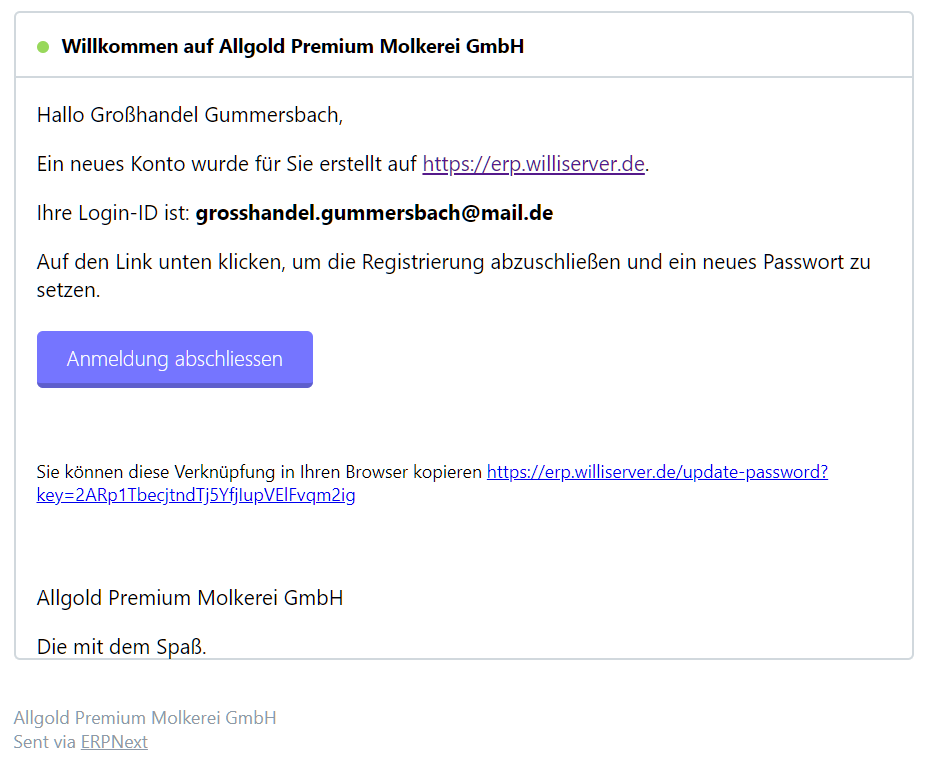
\includegraphics[width=\textwidth]{Bilder/Registrierung_Mail.PNG}
  \caption{Bestätigung der Registrierung per Email}
  \label{fig:regMail}
\end{figure}
\begin{figure}[H]
  \centering
  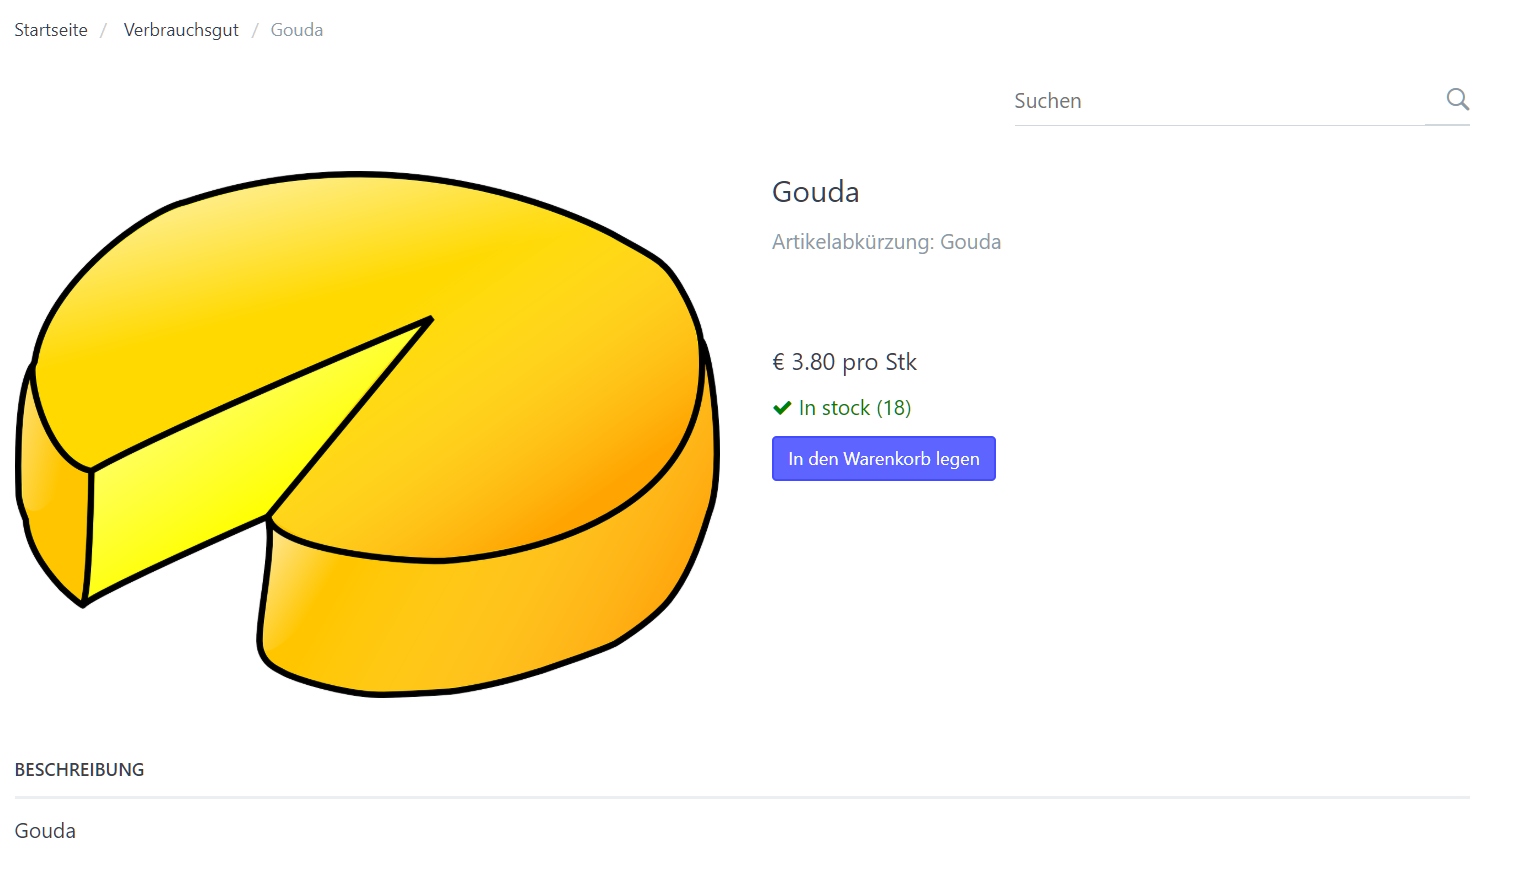
\includegraphics[width=\textwidth]{Bilder/Webshop_Gouda.PNG}
  \caption{Produkt Gouda im Webshop}
  \label{fig:webGouda}
\end{figure}
\begin{figure}[H]
  \centering
  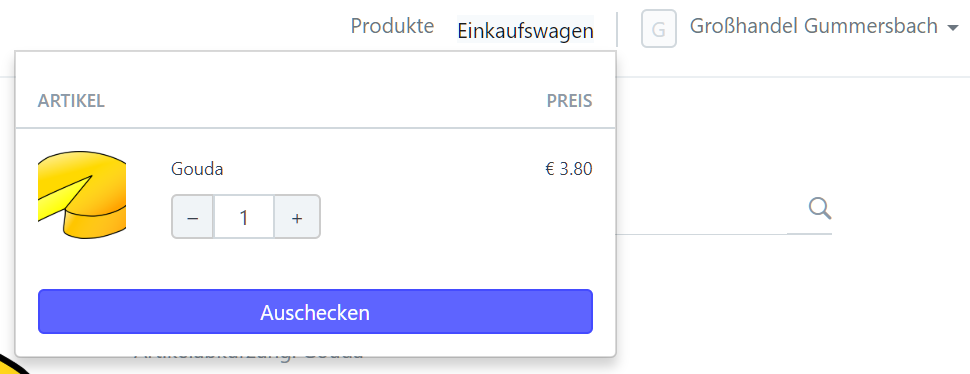
\includegraphics[width=\textwidth]{Bilder/Einkaufswagen.PNG}
  \caption{Einkaufswagen des Webshops}
  \label{fig:webChart}
\end{figure}
\begin{figure}[H]
  \centering
  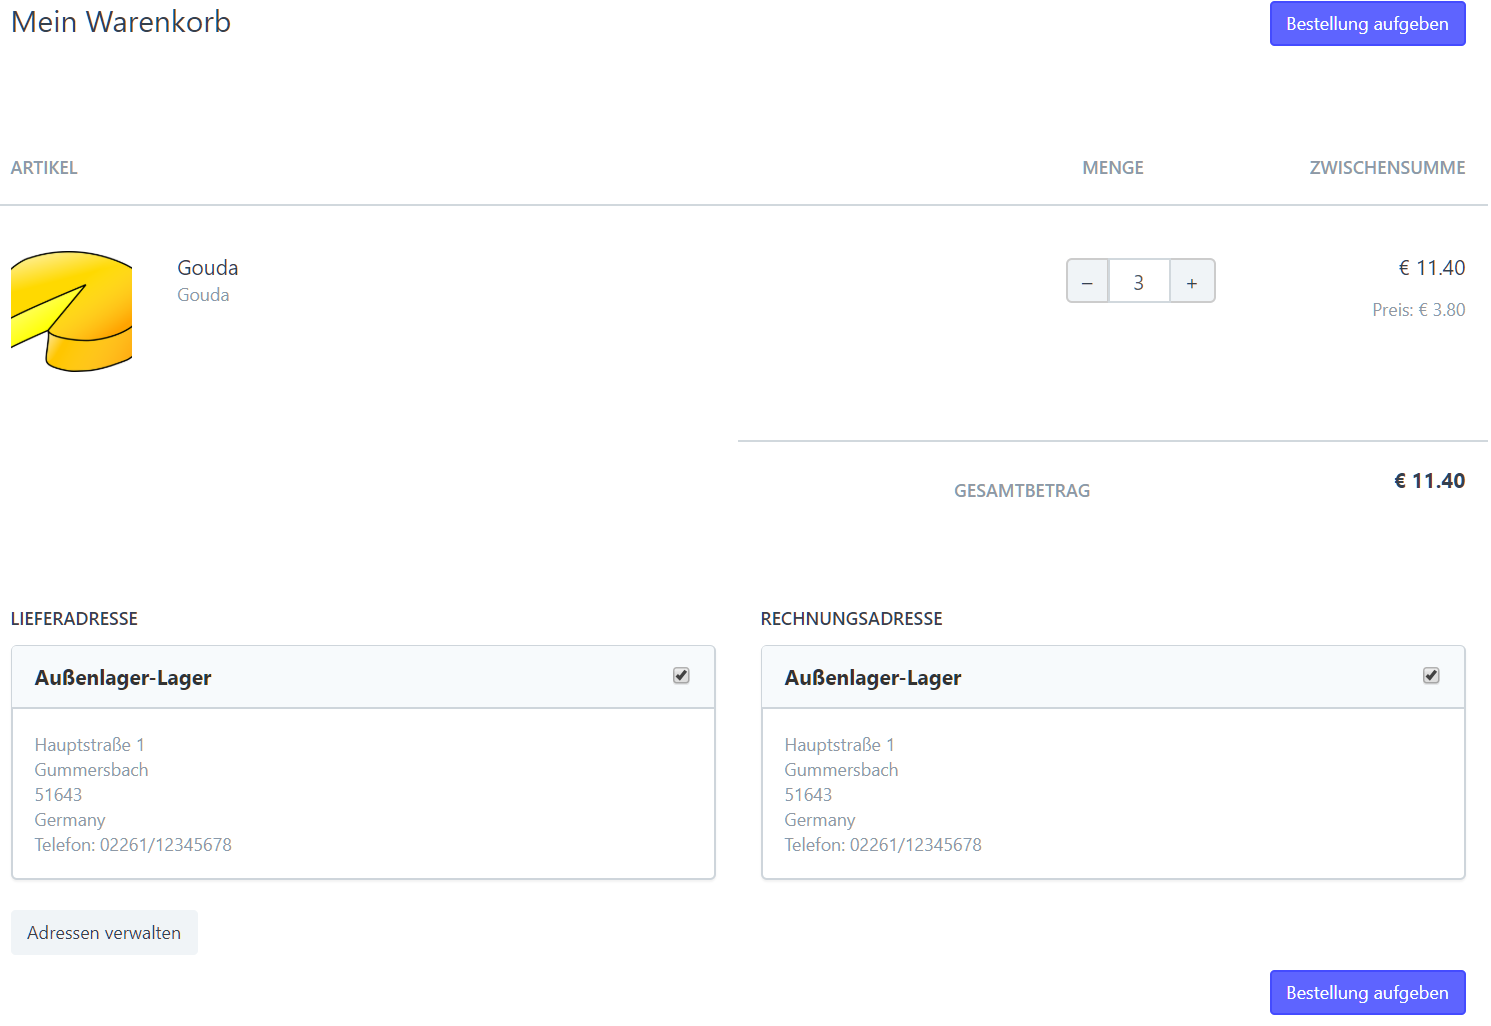
\includegraphics[width=\textwidth]{Bilder/Bestellung.PNG}
  \caption{Warenkorb mit Adressen des Kunden}
  \label{fig:webWarenkorb}
\end{figure}
\begin{figure}[H]
  \centering
  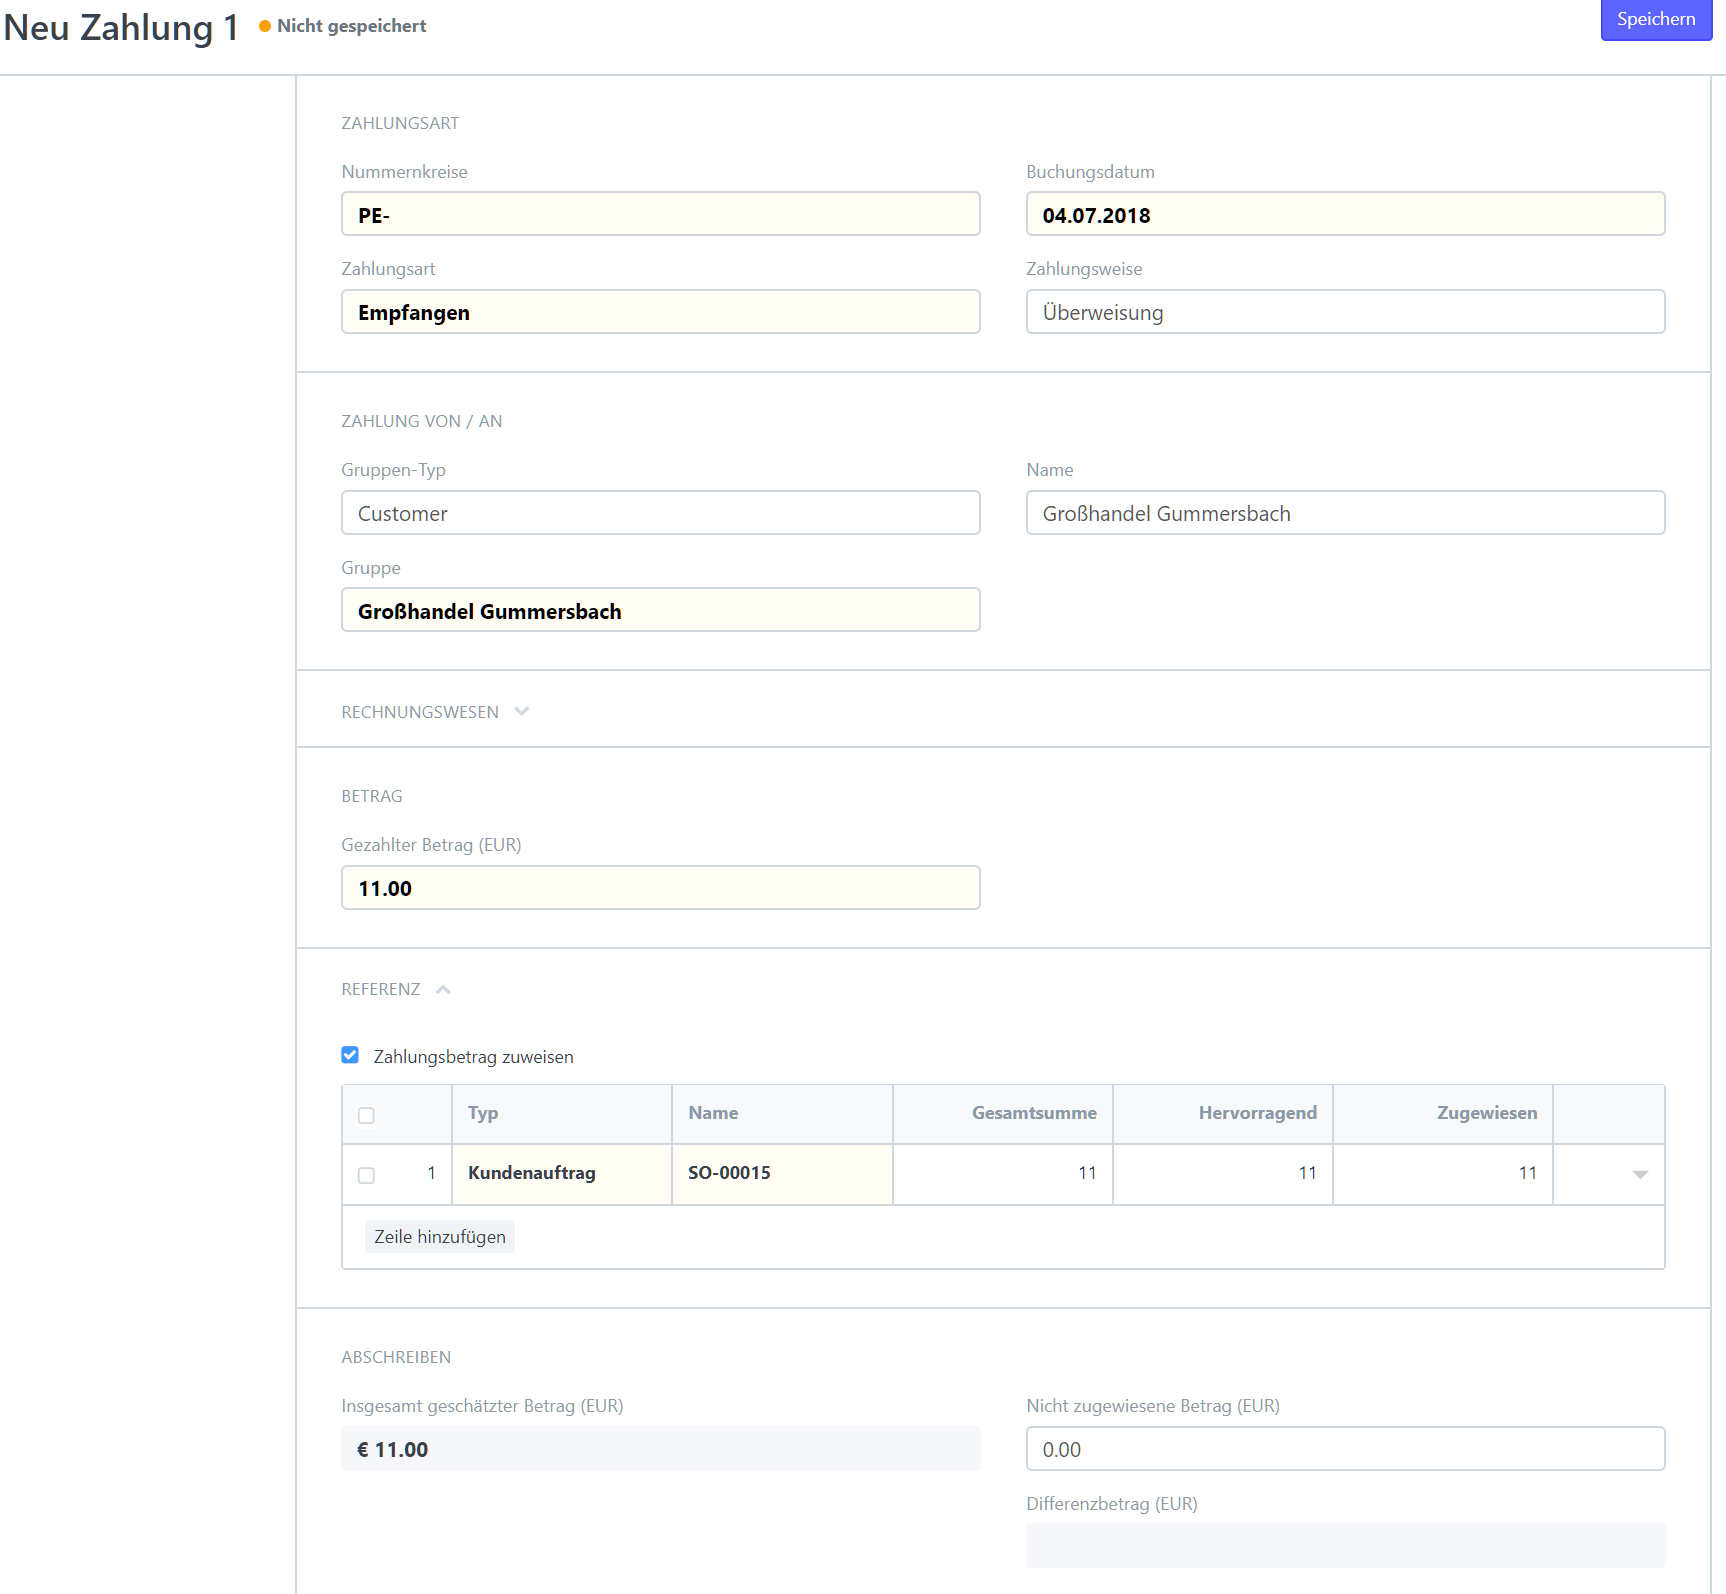
\includegraphics[width=\textwidth]{Bilder/Zahlung_Kunde.PNG}
  \caption{Zahlung des Kunden}
  \label{fig:zahKunde}
\end{figure}
\begin{figure}[H]
  \centering
  
\includegraphics[width=\textwidth]{Bilder/JS_Popup.PNG}
  \caption{Programmiertes JavaScript-Popup}
  \label{fig:jsPopup}
\end{figure}
\begin{figure}[H]
  \centering
  
\includegraphics[width=\textwidth]{Bilder/Fehlermeldung.PNG}
  \caption{Fehlermeldung beim Systemabsturz}
  \label{fig:fehlMeldung}
\end{figure}

